	%%%%%%%%%%%%%%%%%%%%%%%%%%%%%%%%%%%%%%%%%%%%%%%%%%%%%%%%%%%%%%%%%%%%%%%%%%%%%%%%
%                         FORMATO DE TESIS FC UNAM                             %
%%%%%%%%%%%%%%%%%%%%%%%%%%%%%%%%%%%%%%%%%%%%%%%%%%%%%%%%%%%%%%%%%%%%%%%%%%%%%%%%
% based on Harish Bhanderi's PhD/MPhil template, then Uni Cambridge
% http://www-h.eng.cam.ac.uk/help/tpl/textprocessing/ThesisStyle/
% corrected and extended in 2007 by Jakob Suckale, then MPI-iCBG PhD programme
% and made available through OpenWetWare.org - the free biology wiki

%                     Under GNU License v3

% ADAPTADO PARA FI-UNAM:  Jesús Velázquez y Marco Ruiz
\sloppy
\documentclass[twoside,11pt]{Latex/Classes/PhDthesisPSnPDF} 
\usepackage{blindtext}
\usepackage[spanish]{babel}
\usepackage{babelbib}
%\usepackage{multicols}
\usepackage{natbib} 
\usepackage{hyperref}
\usepackage{url}
\usepackage{hyperref}
\usepackage{breakurl}
%\usepackage[dvips]{graphicx}
\usepackage{graphicx}
\usepackage{fancyhdr}
\usepackage{multicol}
\usepackage{mathtools}
\usepackage{float}
\usepackage{theorem}
\setlength{\theorempreskipamount}{5mm}
\setlength{\theorempostskipamount}{5mm}
\theoremstyle{break}
\theorembodyfont{\normalfont}
\theoremheaderfont{\scshape}
\newtheorem{thm}{\bf \textit{Teorema} }
\newtheorem{lem}{\bf \textit{Lema}    }
\newtheorem{defini}{\bf \textit{Definición}    }
\newtheorem{corola}{\bf \textit{Corolario}    }
\usepackage{algorithm}
\usepackage{algpseudocode}
\usepackage[all]{xy} %paquete de diagramas
\setcitestyle{square}
%\usepackage{lipsum}% http://ctan.org/pkg/lipsum
%\usepackage{showframe}% http://ctan.org/pkg/showframe
%\usepackage{eso-pic}% http://ctan.org/pkg/eso-pic
\usepackage{graphicx}% http://ctan.org/pkg/graphicx
%\usepackage{algorithm2e}
%[ruled,vlined,lined,linesnumbered,algochapter,portugues]

\makeatletter
\def\BState{\State\hskip-\ALG@thistlm}
\makeatother

                     % Para insertar texto dummy, de ejemplo, pues.
% Note:
% The \blindtext or \Blindtext commands throughout this template generate dummy text
% to fill the template out. These commands should all be removed when 
% writing thesis content.
% This file contains macros that can be called up from connected TeX files
% It helps to summarise repeated code, e.g. figure insertion (see below).

%%%%%%%%%%%%%%%%%%%%%%%%%%%%%%%%%%%%%%%%%%%%%%
%            Colores de la UNAM              %
%%%%%%%%%%%%%%%%%%%%%%%%%%%%%%%%%%%%%%%%%%%%%%
%Azul Pantone 541  -->(0,63,119) RGB
\definecolor{Azul}{RGB}{0,63,119}

%Oro Pantone 460  -->(234,221,150) RGB
\definecolor{Oro}{RGB}{234,221,150}


%%%%%%%%%%%%%%%%%%%%%%%%%%%%%%%%%%%%%%%%%%%%%%
%            Comandos para líneas            %
%%%%%%%%%%%%%%%%%%%%%%%%%%%%%%%%%%%%%%%%%%%%%%
%Se define un comando \colorvrule para hacer líneas verticales de color con 3 argumentos: color, ancho, alto
\newcommand{\colorvrule}[3]{
\begingroup\color{#1}\vrule width#2 height#3
\endgroup}

%Se define un comando \colorhrule para hacer líneas horizontales de color con 2 argumentos: color, ancho
\newcommand{\colorhrule}[2]{
\begingroup\color{#1}\hrule height#2
\endgroup}

%%%%%%%%%%%%%%%%%%%%%%%%%%%%%%%%%%%%%%%%%%%%%%
%          Comando para derivadas            %
%%%%%%%%%%%%%%%%%%%%%%%%%%%%%%%%%%%%%%%%%%%%%%
\newcommand{\derivada}[3][]{\ensuremath{\dfrac{\mbox{d}^{#1}#2}{\mbox{d}#3^{#1}}}} 
%primer argumento(opcional): orden de la derivada
%segundo argumento: función a derivar
%tercer argumento: variable respecto a la que se deriva


%%%%%%%%%%%%%%%%%%%%%%%%%%%%%%%%%%%%%%%%%%%%%%
%       Comando para la exponencial          %
%%%%%%%%%%%%%%%%%%%%%%%%%%%%%%%%%%%%%%%%%%%%%%
\newcommand{\e}[1][]{\ensuremath{\mbox{e}^{#1}}}
%primer argumento(opcional): exponente de la exponencial




% insert a centered figure with caption and description
% parameters 1:filename, 2:title, 3:description and label
\newcommand{\figuremacro}[3]{
	\begin{figure}[htbp]
		\centering
		\includegraphics[width=1\textwidth]{cabezaaa}
		\caption[#2]{\textbf{#2} - #3}
		\label{condicion}
	\end{figure}
}

% insert a centered figure with caption and description AND WIDTH
% parameters 1:filename, 2:title, 3:description and label, 4: textwidth
% textwidth 1 means as text, 0.5 means half the width of the text
\newcommand{\figuremacroW}[4]{
	\begin{figure}[htbp]
		\centering
		\includegraphics[width=#4\textwidth]{#1}
		\caption[#2]{\textbf{#2} - #3}
		\label{#1}
	\end{figure}
}

% inserts a figure with wrapped around text; only suitable for NARROW figs
% o is for outside on a double paged document; others: l, r, i(inside)
% text and figure will each be half of the document width
% note: long captions often crash with adjacent content; take care
% in general: above 2 macro produce more reliable layout
\newcommand{\figuremacroN}[3]{
	\begin{wrapfigure}{o}{0.5\textwidth}
		\centering
		\includegraphics[width=0.7\textwidth]{#1}
		\caption[#2]{{\small\textbf{#2} - #3}}
		\label{#1}
	\end{wrapfigure}
}

% predefined commands by Harish
\newcommand{\PdfPsText}[2]{
  \ifpdf
     #1
  \else
     #2
  \fi
}

\newcommand{\IncludeGraphicsH}[3]{
  \PdfPsText{\includegraphics[height=#2]{#1}}{\includegraphics[bb = #3, height=#2]{#1}}
}

\newcommand{\IncludeGraphicsW}[3]{
  \PdfPsText{\includegraphics[width=#2]{#1}}{\includegraphics[bb = #3, width=#2]{#1}}
}

\newcommand{\InsertFig}[3]{
  \begin{figure}[!htbp]
    \begin{center}
      \leavevmode
      #1
      \caption{#2}
      \label{#3}
    \end{center}
  \end{figure}
}






%%% Local Variables:
%%% mode: latex
%%% TeX-master: "~/Documents/LaTeX/CUEDThesisPSnPDF/thesis"
%%% End:
           % Archivo con funciones útiles
%%%%%%%%%%%%%%%%%%%%%%%%%%%%%%%%%%%%%%%%%%%%%%%%%%%%%%%%%%%%%%%%%%%%%%%%%%%%%%%%
%                                   DATOS                                      %
%%%%%%%%%%%%%%%%%%%%%%%%%%%%%%%%%%%%%%%%%%%%%%%%%%%%%%%%%%%%%%%%%%%%%%%%%%%%%%%%
\title{Método de parametrización: Variedades estables e inestables en mapeos hamiltonianos de dos dimensiones}
\author{\LARGE Evelyn Álvarez Cruz}        
\degree{Física}               % Carrera
\director{Dr. Luis Benet Fernández}               % Director de tesis
\degreedate{2019}                           % Año de la fecha del examen
\lugar{México, D.F.}                        % Lugar
%\portadafalse                              % Portada en NEGRO, descomentar y comentar la línea siguiente si se quiere utilizar
\portadatrue                                % Portada en COLOR

\keywords{tesis,autor,tutor,etc}            % Palablas clave para los metadatos del PDF
\subject{tema_1,tema_2}    

           % Tema para metadatos del PDF  

%%%%%%%%%%%%%%%%%%%%%%%%%%%%%%%%%%%%%%%%%%%%%%%%%%%%%
%                   PORTADA                         %
%%%%%%%%%%%%%%%%%%%%%%%%%%%%%%%%%%%%%%%%%%%%%%%%%%%%%
\begin{document}
\maketitle									% Se redefinió este comando en el archivo de la clase para generar automáticamente la portada a partir de los datos

%%%%%%%%%%%%%%%%%%%%%%%%%%%%%%%%%%%%%%%%%%%%%%%%%%%%%
%                  PRÓLOGO                          %
%%%%%%%%%%%%%%%%%%%%%%%%%%%%%%%%%%%%%%%%%%%%%%%%%%%%%
\frontmatter
\begin{dedication}
A mis padres
\end{dedication}
 
% ******************************* Thesis Declaration ********************************

\begin{declaration}

Por la presente declaro que, salvo cuando se haga referencia específica al trabajo de otras personas, el contenido de esta tesis es original y no se ha presentado total o parcialmente para su consideración para cualquier otro título o grado en esta o cualquier otra Universidad. Esta tesis es resultado de mi propio trabajo y no incluye nada que sea el resultado de algún trabajo realizado en colaboración, salvo que se indique específicamente en el texto. 
% Author and date will be inserted automatically from thesis.tex

\end{declaration}
  
%\chapter*{}
%\pagenumbering{Roman}

\begin{acknowledgements}

También quisiera reconocer a ... por ...CONACYT,  PAPIIT / etc.
\blindtext % Dummy text
\end{acknowledgements}




     % Comentar línea si no se usa

\chapter{Introducción}
En el análisis de sistemas dinámicos es importante desarrollar aspectos que nos ayuden a describir de manera puntual el comportamiento de un sistema, esto ya que muchos de ellos tienen una dinámica rica en el sentido matemático y físico. Conocer por ejemplo los puntos fijos, las órbitas periódicas, el diagrama de bifurcación, entre otras características es una manera de poder decir mucho sobre el sistema en general. Entre esas características está el estudio de las variedades estables e inestables alrededor de puntos fijos o de periodo $n$. La importancia de las variedades radica en que mediante éstas se puede conocer el comportamiento del sistema dinámico en las vecindades del punto periódico, además para algunos casos la intersección de las mismas lleva a resultados interesantes sobre caos. Se puede por ejemplo estudiar el problema de los tres cuerpos mediante el estudio de sus variedades cerca del punto fijo, haciendo una linearización del problema.\\


El estudio analítico de las variedades cerca de puntos periódicos (puntos fijos y de periodo igual o mayor a dos) se ha complementado con el numérico. Dentro de los métodos semianalíticos se encuentra el de parametrización \citep{Haro}. El método de parametrización, dicho de manera simple consiste en aproximar mediante series de Taylor las variedades alrededor de puntos periódicos usando que las variedades son solución a la ecuación de invariancia. Los coeficientes de los polinomios de Taylor se van calculando de manera recursiva. El método se describe en el trabajo de J.D. Mireles \citep{Mireles}, quién  lo aplicó de manera particular al mapeo estándar, describiendo muy claramente cómo se obtienen las relaciones de recurrencia; su trabajo es la motivación de esta tesis.\\


El objetivo de este trabajo es ir más allá de implementar el método de parametrización para el mapeo estándar. Siguiendo las notas mencionadas se automatizó el método de manera computacional primero para el mapeo estándar y luego se hizo de manera general para cualquier mapeo de dos dimensiones. Con el método implementado se obtienen las variedades estable e inestable alrededor de puntos fijos hiperbólicos, parametrizadas por medio de un polinomio de orden $n$.
Teniendo las variedades se hizo un análisis de las intersecciones entre ellas y de cómo explotar el método para mejorar el error.
 
Este escrito se divide en tres partes. En el primer capítulo presentaré la teoría de los sistemas dinámicos Hamiltonianos que se usará a lo largo del método, junto con el método de parametrización. Primero introducimos qué es un sistema dinámico junto con las definiciones de puntos fijos y órbitas periódicas, llegando a la teoría detrás de la ecuación de invariancia. Las matemáticas que se utilizan en el proceso de parametrización están al alcance de un estudiante de licenciatura de Física o Matemáticas, sin embargo la teoría detrás del funcionamiento del método es un tanto más elevada de nivel, por lo que sólo mencionaremos en esta parte las herramientas más fundamentales.  \\


En el segundo capítulo pasaremos a describir brevemente cómo J.D Mireles aplica el método para un caso particular para posteriormente explicar cómo se procedió a implementar el método. En esta parte también se incluye el análisis del error y de la convergencia de las soluciones. El tercer y último capítulo consiste en analizar el mapeo estándar para reproducir algunos de los resultados presentados en \cite{Mireles}. También se analizarán otros mapeos como el de Hénon y el que aparece en el artículo \cite{Jung}. Por último se presenta una breve perspectiva en la que mencionamos algunas de las ideas con las que se podría seguir trabajando a partir del método automatizado. \\

Dado que es un trabajo semianalítico se incluirán algunos enlaces que llevarán a ejemplos o códigos que se usen dentro del programa, con la documentación correspondiente. También hay algunas partes interactivas que estarán en línea. 

            % ~10 páginas - Explicar el propósito de la tesis
  % Comentar línea si no se usa 
%% ******************************* Thesis Declaration ********************************

\begin{declaration}

Por la presente declaro que, salvo cuando se haga referencia específica al trabajo de otras personas, el contenido de esta tesis es original y no se ha presentado total o parcialmente para su consideración para cualquier otro título o grado en esta o cualquier otra Universidad. Esta tesis es resultado de mi propio trabajo y no incluye nada que sea el resultado de algún trabajo realizado en colaboración, salvo que se indique específicamente en el texto. 
% Author and date will be inserted automatically from thesis.tex

\end{declaration}
           % Comentar línea si no se usa
%
% Thesis Abstract -----------------------------------------------------


%\begin{abstractslong}    %uncommenting this line, gives a different abstract heading
\begin{abstracts}        %this creates the heading for the abstract page

This is where you write your abstract ...
\blindtext

\end{abstracts}
%\end{abstractlongs}


% ----------------------------------------------------------------------                   % Comentar línea si no se usa

%%%%%%%%%%%%%%%%%%%%%%%%%%%%%%%%%%%%%%%%%%%%%%%%%%%%%
%Esta sección genera el índice
\setcounter{secnumdepth}{3} % organisational level that receives a numbers%                   ÍNDICES                         %
%%%%%%%%%%%%%%%%%%%%%%%%%%%%%%%%%%%%%%%%%%%%%%%%%%%%%
\setcounter{tocdepth}{3}    % print table of contents for level 3
\tableofcontents            % Genera el índice 
%: ----------------------- list of figures/tables ------------------------
%\listoffigures              % Genera el ínidce de figuras, comentar línea si no se usa
%\listoftables               % Genera índice de tablas, comentar línea si no se usa


%%%%%%%%%%%%%%%%%%%%%%%%%%%%%%%%%%%%%%%%%%%%%%%%%%%%%
%                   CONTENIDO                       %
%%%%%%%%%%%%%%%%%%%%%%%%%%%%%%%%%%%%%%%%%%%%%%%%%%%%%
% the main text starts here with the introduction, 1st chapter,...
\mainmatter
\def\baselinestretch{1.5}                   % Interlineado de 1.5
%%%%%%%%%%%%%%%%%%%%%%%%%%%%%%%%%%%%%%%%%%%%%%%%%%%%%%%%%%%%%%%%%%%%%%%%%
%           Capítulo 2: MARCO TEÓRICO - REVISIÓN DE LITERATURA
%%%%%%%%%%%%%%%%%%%%%%%%%%%%%%%%%%%%%%%%%%%%%%%%%%%%%%%%%%%%%%%%%%%%%%%%%
\chapter{Sistemas Hamiltonianos de dos dimensiones}
Para llegar al análisis de los sistemas de nuestro interés mediante el método de parametrización es fundamental conocer algunos conceptos sobre la dinámica así como del análisis numérico del mismo. En este capítulo se hace una breve descripción de los teoremas y definiciones que nos ayudarán a entender el método. Las siguientes secciones no son la manera más formal de introducir al lector a cada uno de los temas expuestos. Sin embargo proporcionan una visión puntual de lo indispensable. 

\section{Sistemas dinámicos}
Cuando uno habla sobre sistemas dinámicos lo que le viene a la mente es alguna relación que describe el comportamiento temporal de un sistema físico. Ya sea el movimiento de péndulos o de cargas, nos interesa saber más acerca de las características de su comportamiento. 
En el estudio de los mismos se hace una clasificación en términos de sus propiedades vistas en el espacio fase o por la forma del sistema. Hay sistemas dinámicos discretos y sistemas dinámicos continuos, en el primero el tiempo varía discretamente mientras que en el segundo varía de manera contínua. \\

 Dentro de estas características de clasificación también puede ser que el sistema sea de tipo determinista o estocástico. La diferencia entre ambos es que para el determinista dado un punto en el espacio fase existe uno y sólo un punto subsecuente bien definido, mientras que en el estocástico para un estado puede haber varios estados subsecuentes posibles.
En algunos casos los sistemas resultan ser simples, por ejemplo si su movimiento es regular. Sin embargo hay muchos otros sistemas que no son regulares en los que para dos condiciones iniciales parecidas los resultados de la dinámica después de cierto tiempo son diferentes. En este trabajo nos enfocaremos en los  sistemas deterministas discretos.\\

Para formalizar usaremos la siguiente definición de sistema dinámico.  \\
\begin{defini}[\textsc{\textit{Sistema dinámico}}\cite{gerald}]
\textit{Un sistema dinámico es un semigrupo $G$ actuando en un espacio $M$, definido por una relación de la forma}
\begin{equation}
T : G \times M \rightarrow M; \quad
T_{g}\circ T_{h}=T_{g\circ h} . \label{def sistema dinamico}
\end{equation}
\end{defini}

Un ejemplo típico de un sistema dinámico continuo es el flujo de una ecuación diferencial autónoma, mientras que de uno discreto es por ejemplo el mapeo de un intervalo cerrado en $\mathbb{R}$ en sí mismo, o simplemente una función iterada. En el primer caso
\begin{equation}
\dot{x} =  f(x); \quad  
x(0)=x_{0} , \label{ec dif}
\end{equation}
suponiendo que $f \in C^{k}(M,\mathbb{R}^{n})$ con $k \geq 1$ y donde $M$ es un subconjunto abierto de $\mathbb{R}^{n}$. Las soluciones de este tipo de sistemas son curvas contenidas en $\mathbb{R}^{n}$ a las que llamamos trayectorias y denotamos por $\phi$.\\
En el segundo caso  
\begin{eqnarray}
\pmb x_{n+1}= \mathbf{f}(\pmb x_{n}) \quad \pmb x\in \mathbb{R}^{n}. \label{sistema discreto}
\end{eqnarray}
Para la ecuación \eqref{sistema discreto} dada una condición inicial $\pmb x_{0}$ podemos obtener el estado siguiente evaluando el lado derecho con tal punto. De manera sucesiva se puede obtener el estado $\pmb x_{n+1}$ del estado $\pmb x_{n}$. La aplicación consecutiva de la función proporciona la trayectoria u órbita del punto inicial. Podemos decir que el mapeo es un isomorfismo entre la condición inicial y los puntos de la trayectoria,
\begin{eqnarray*}
\pmb x_{k}=\mathbf{f}\circ\mathbf{f}\circ \mathbf{f} \circ \mathbf{f} ... \circ \mathbf{f} (\pmb x_{0})\quad (k \quad \textrm{veces})
\end{eqnarray*}
o
\begin{eqnarray*}
\pmb x_{k} = \mathbf{f}^{k}(\pmb x_{0}).
\end{eqnarray*}
Al conjunto $\lbrace \pmb x_{0},\pmb x_{1},...,\pmb x_{n} \rbrace$ se le llama la órbita de $\pmb x_{0}$.  En este tipo de sistemas es posible que exista un $\pmb x_{*}$ tal que $\mathbf{f}^{p}(\pmb x_{*})=\pmb x_{*}$ con $p \in \mathbb{Z}$. Es decir después de un número finito de aplicaciones se vuelve al mismo punto ($\pmb x_{*}$) al cual le llamamos un punto de periodo $p$. También es entonces posible  que exista un punto de periodo uno $\pmb x_{*}=\mathbf{f}(\pmb x_{*})$ al cual llamamos punto fijo. Los puntos fijos serán otra forma de clasificar a los sistemas dinámicos, para ello separamos las órbitas en términos de los periodos:

\begin{itemize}
\item  Órbitas fijas (asociadas a puntos con periodo uno).
\item Órbitas periódicas regulares (asociadas a puntos con periodo mayor a uno).
\item Órbitas no cerradas (asociadas a puntos no periódicos).
\end{itemize}
Nos enfocaremos sobre todo en los puntos fijos, sin embargo es posible también analizar aquellos puntos de periodo mayor a uno.
\section{Mapeos}
Como mencionamos en la introducción existen diferentes características de los sistemas dinámicos, la forma en la que depende un estado del estado anterior es una de ellas. Esa dependencia está determinada por $\mathbf{f}$ en la ecuación \eqref{sistema discreto}; gráficamente se describe en el espacio fase, que es el espacio de todos los posibles valores de $\pmb x$. En el mismo espacio la órbita de cualquier punto se ve como una trayectoria que representa la evolución de un punto $\pmb x$ bajo el mapeo hacia adelante y hacia atrás. \\

Las funciones que aparecen en el mapeo pueden contener términos con potencia mayor a uno, productos entre las variables o peor aún funciones mucho más difíciles de manejar, lo que hace que la suma de soluciones no sea solución, esa característica se llama no linealidad. Una de las primeras cosas a analizar serían los puntos fijos del sistema, los cuales deberán encontrarse algebráicamente o numéricamente dependiendo de la dificultad del mapeo, al rededor de los cuales pueden presentarse diversos comportamientos de las trayectorias.\\

Si tenemos un puno fijo $\mathbf{x}_{*}$ asociado al mapeo entonces la ecuación
\begin{eqnarray}
\mathbf{x}_{n+1} =\mathbf{A}\mathbf{x}_{n},
\end{eqnarray}
representa el sistema linearizado alrededor del punto, donde $\mathbf{A}=D\mathbf{f}(\mathbf{x}_{*})$. Es decir el mapeo puede ser representado como una matriz de coeficientes constantes,además si el sistema dinámico es invertible se puede conocer el punto anterior $\mathbf{x}_{n-1}$ a un cierto $\mathbf{x}_{n}$ usando la matriz inversa de $\mathbf{A}$ que representa la linearización del mapeo inverso $\mathbf{f}^{-1}$. Es decir las características de tal matriz nos dirán el comportamiento del sistema. \\

Dado que los sistemas tratados en este trabajo son de dos dimensiones entonces analizaremos sólo este caso. Los valores propios $\lambda_{1}, \lambda_{2}$, soluciones del polinomio característico de grado dos, son en general valores complejos clasificados como sigue.
\begin{itemize}
\item $\vert \lambda_{i}\vert<1$
\item $\vert \lambda_{i}\vert>1$
\item $\vert \lambda_{i}\vert=1$
\end{itemize}
En cada uno de los casos anteriores tenemos un vector propio $\mathbf{x}_{p1}$ asociado, tal que 
\begin{eqnarray}
\mathbf{A}\mathbf{x}_{p1}=\lambda_{1}\mathbf{x}_{p1}.
\end{eqnarray}
Los vectores serán linealmente independientes si $\lambda_{1},\lambda_{2}$ son diferentes. Si además consideramos que los valores propios son reales, según \cite{Friedberg} existe una matriz $\mathbf{U}$ tal que 
\begin{eqnarray}
\mathbf{U}^{-1}\mathbf{A}\mathbf{U} = \begin{pmatrix}
\lambda_{1} & 0\\
0 & \lambda_{2}\\
\end{pmatrix}.
\end{eqnarray}
A partir de esto es fácil ver que $\mathbf{U}$ tiene como columnas los vectores propios. Consecuentemente un mapeo lineal de dimensión dos es linealmente conjugado con un mapeo el cual tiene una matriz de representación diagonal. Este tipo de matrices son llamadas formas normales y
permiten representar el sistema en su forma más simple mediante la diagonalización del mismo \citep{arnold}.\\

Cuando $\mathbf{A}$ es una matriz diagonalizable y sus valores propios son puramente imaginarios entonces decimos que el punto fijo tiene un comportamiento elíptico. Si es el caso que ninguno de los dos valores propios tienen parte real cero entonces el punto fijo asociado es un punto fijo hiperbólico. El resultado de estas características visto en el espacio fase es un comportamiento muy particular que se muestra en la figura \ref{hiperbolic}. \\

\begin{figure}[h!]
\centering
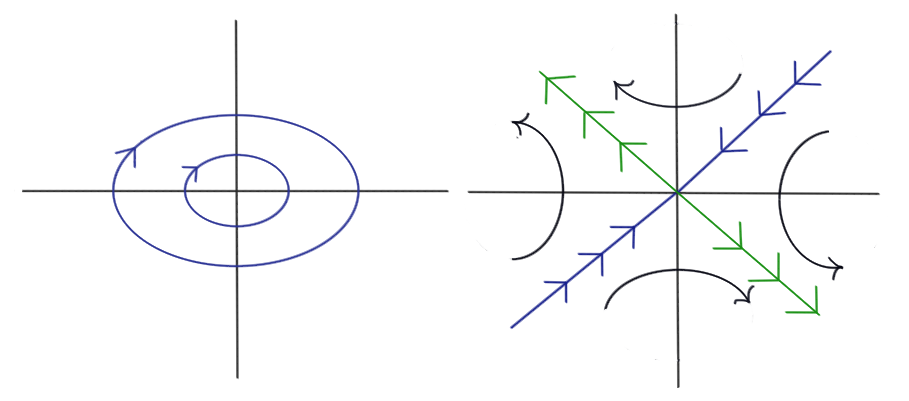
\includegraphics[scale=0.3]{hyperbolic} 
\caption{Punto fijo elíptico(izquierda) e hiperbólico(derecha) en el espacio fase.}
\label{hiperbolic}
\end{figure}


%Retomando además que si los valores propios eran ortogonales entonces podemos escribir los subespacios generados por los vectores propios.
%\begin{eqnarray*}
%E^{s}=\lbrace (x,y) : (x,y)=\beta \pmb v_{1} \quad \beta\in \mathbb{R}\rbrace
%\end{eqnarray*}
%\begin{eqnarray*}
%E^{u}=\lbrace (x,y) : (x,y)=\alpha \pmb v_{2}\quad \alpha\in \mathbb{R}\rbrace
%\end{eqnarray*}

En el caso hiperbólico tenemos dos comportamientos que nos interesan, marcados con las líneas azul y verde de la figura \ref{hiperbolic}, tales corresponden a los eigenespacios asociados a los vectores propios de $\mathbf{A}$. Existe un teorema importante de Hartman-Grobman que nos asegura que hay una vecindad del punto fijo hiperbólico tal que el mapeo es topológicamente conjugado a su linearización \cite{Meiss,Meyer,Juergen}. Dicho de otra manera, hay vecindades $U$ de $\mathbf{x}_{*}$, $V$ de $0 \in \mathbf{R}^{2}$ y un homeomorfismo $h:U\rightarrow V$ tal que $h$ mapea trayectorias de $\mathbf{f}$ en trayectorias del sistema lineal. De esta manera justificamos el porque se trabaja con un sistema lineal.



\section{Conjuntos invariantes}
Alrededor de un punto fijo existen ciertos conjuntos que nos dirán algunas características del sistema; estos conjuntos tienen que ver directamente con lo que se observa en la figura \ref{hiperbolic}. Para entender su comportamiento necesitamos definir qué es un conjunto invariante.

\begin{defini}[\textit{\textsc{Conjunto invariante}}\cite{Ott}]
\textit{Un conjunto invariante es un subconjunto $\mathbf{I} \subset \mathbf{E}$ del espacio fase tal que para cualquier $\mathbf{x}_{i}\in  \mathbf{I}$  y $ n\in\mathbb{N}$ \\
\begin{center}
$\mathbf{f}^{n}(\mathbf{x}_{i}) \in \mathbf{I}$.
\end{center}
}
\end{defini}
Es decir que cualquier elemento tomado en el conjunto se queda en el conjunto bajo la aplicación del mapeo. \\
Estudiaremos los conjuntos invariantes asociados a puntos fijos hiperbólicos. Si $\mathbf{x}_{*}$ es un punto fijo hiperbólico entonces definimos las variedades estable e inestable como
\begin{eqnarray}
W^{s}=\lbrace \mathbf{x} : \mathbf{f}^{n}(\mathbf{x})\rightarrow \mathbf{x}_{*} \quad cuando \quad n\rightarrow \infty \rbrace
\label{variedad estable}
\end{eqnarray}

\begin{eqnarray}
W^{u}=\lbrace \mathbf{x} : \mathbf{f}^{n}(\mathbf{x})\rightarrow \mathbf{x}_{*} \quad cuando \quad n\rightarrow -\infty \rbrace.
\label{variedad inestable}
\end{eqnarray}


Localmente las variedades resultan ser tangentes a los subespacios generados por los vectores propios

\begin{eqnarray*}
E^{s}=\lbrace (x,y) : (x,y)=\beta \pmb v_{1} \quad \beta\in \mathbb{R}\rbrace,
\end{eqnarray*}
\begin{eqnarray*}
E^{u}=\lbrace (x,y) : (x,y)=\alpha \pmb v_{2}\quad \alpha\in \mathbb{R}\rbrace .
\end{eqnarray*}
Esto se resume en el siguiente teorema.


%\begin{defini}[Variedad estable e inestable para un punto fijo]
%Sea \textit{$F:\mathbb{R}^{2}\rightarrow\mathbb{R}^{2}$ un  mapeo y sea $\pmb x_{*}$ un punto fijo %del mapeo , si $C \in \mathbb{R}^{2}$ es una vecindad del punto fijo  definimos}
%\begin{eqnarray*}
%W_{loc}^{s}(\pmb x_{*})=\lbrace \epsilon \in  C : \mathbf{F}^{n}(\pmb x_{i}) \in C \quad \forall n\in \mathbb{N} \rbrace
%\end{eqnarray*}
%\label{Variedad  defini}
%\end{defini}
%la definición $4$ es análoga para la variedad inestable $W_{loc}^{u}$ , pero sólo nos da una relación local. Si queremos ir más alejados del punto fijo entonces necesitamos una variedad que sea más general.Para ello existe el teorema siguiente.
%\begin{thm}[De la variedad estable(inestable)]
%\textit{Sea $\mathbf{A}$ una matriz de $2\times 2$ con dos valores propios $\lambda_{1},\lambda_{2}$ donde uno tiene parte real positiva y otro negativa, tal que si $\epsilon $ es lo suficientemente pequeña y positiva existe $ W^{s}(\pmb x_{i})$  entonces $F^{n}(\pmb x_{i})\rightarrow x_{*}$ cuando $n\rightarrow\infty$.  Respectivamente para $W^{u}(\pmb x_{i}
%)$ tenemos que $F^{n}(\pmb x_{i})\rightarrow x_{*}$ cuando $n\rightarrow -\infty$. }
%\end{thm}






%Con esto podemos asegurarar que existen funciones lo sificientemente suaves que se extienden por la %variedad, no solo de manera local. Esto es de suma importancia en el método de parametrización que %aplicaremos,ya que la parametrización se hace por medio de polinomios que son funciones suaves y %que con lo que acabamos de mencionar no sólo se aproximan de manera local. Si escribimos el %conjunto de la definición anterior
%\begin{eqnarray}
%W^{s}(\pmb x_{i})=\lbrace \pmb x_{i} \in \mathbb{R}^{2}: \lim_{n\rightarrow\infty} \mathbf{F}^{n}%(\pmb x_{i}) =x_{*}\rbrace \label{omega s}
%\end{eqnarray}
%podemos notar que además tal conjunto consiste en todas las órbitas que se acumulan bajo la %aplicación iterada del mapeo al punto fijo. En el caso en que el mapeo se a invertible entonces %podemos relacionar 
%\begin{eqnarray*}
%W^{s}(\pmb x_{*})=\cup_{n=0}^{\infty}\mathbf{F}^{n}[W_{loc}^{s}(\pmb x_{i})]
%\end{eqnarray*}
%que nos dice que la variedad estable se obtiene de la union de todas las aplicaciones hacia atrás de la variedad local estable. Para escribir de manerá análoga la variedad inestable digamos primero que la órbita hacia atrás de $\pmb x_{k}$  es $\mathbf{F}(\pmb x_{k})=\pmb x_{k+1}$ con $k\leq -1 $ donde además
%\begin{eqnarray*}
%\lim_{k\rightarrow -\infty} \pmb F(\pmb x_{k})=x_{*}
%\end{eqnarray*}
%si el mapeo es invertible entonces la órbita hacia atrás es simplemente la aplicación iterada de la %inversa. Entonces
%\begin{eqnarray*}
%W^{u}(\pmb x_{*})=\lbrace \pmb x_{i} \in \mathbb{R}^{2}: \lim_{n\rightarrow\infty} \pmb F^{n}(\pmb %x_{i})=\pmb x_{*}\rbrace \label{omega u}
%\end{eqnarray*}

%Para relacionar esto con los sistemas de interés regresemos a la ecuación \ref{sistema discreto} %donde es evidente que el origen $[0,0]$ es un punto fijo de cualquier sistema que tenga la misma forma. Si ninguno de los dos eigenvalores $\lambda_{1,2}$ de la matriz $\mathbb{A}$ tiene módulo uno  y se tiene que ambos son de signo contrario entonces la matriz es llamada hiperbólica y $x_{*}$ un punto fijo hiperbólico. Mientras que si por ejemplo los dos valores propios de $A$ tienen solo parte imaginaria entonces el sistema es llamado elíptico. El comportamiento de ambos casos se puede ver en la figura \ref{hiperbolic}. Estos conjuntos invariantes relacionados con el punto fijo resultan ser espacios propios generalizados de la matriz $\mathbb{A}$ generados por los vectores propios. Es decir si $\pmb x_{pj}=\pmb u_{j}+i\pmb v_{j}$ proviene de una base 
%\begin{eqnarray}
%\mathbf{B}=\lbrace \pmb u_{1},\pmb v_{1},\pmb u_{2},\pmb v_{2} \rbrace
%\end{eqnarray}
%entonces hay diferentes direcciones asociadas al punto fijo de acuerdo con la base $\mathbf{B}$. Para los sistemas que trabajaremos resulta que no sólo la norma de los valores propios son menores o mayores a uno, si no que además la parte imaginaria es cero para ambos. Lo que quiere decir que la base $\mathbf{B}$ tiene dos elementos únicamente. Los elementos de la misma forman subespacios, un subespacio asociado al valor propio con norma mayor a uno y otro con norma menor a uno. 

%Tomado de MAteo wirth
%\begin{thm}
%\textit{Dado un sistema de la forma \ref{sistema discreto} donde los valores propios de $\mathbb{A}$ tengan parte real diferente de cero entonces}
%\begin{eqnarray*}
%W^{s} = E^{s} 
%\end{eqnarray*}
%\begin{eqnarray*}
%W^{u}=E^{u}
%\end{eqnarray*}
%\end{thm}
%\textit{donde $E^{s}$ es la suma directa de los eigenespacios asociados al valor propio con parte real negativa , $E^{u}$ es análogo pero con positivo. En particular}
%\begin{eqnarray*}
%\mathbb{R}^{n}= W^{s}\oplus W^{u}
%\end{eqnarray*}

%Puesto que los valores propios son reales,  y entonces también los vectores propios. Este teorema nos resume que la suma directa de los conjuntos invariantes del sistema forman al espacio de soluciones. Además de mostrarnos que los conjuntos invariantes son para este caso las variedades invariantes. En el caso de sistemas más generales tenemos el siguiente teorema, que además nos aclara a qué llamamos una variedad inestable. \\


\begin{thm}[\underline{\textit{De la variedad estable}} \cite{Mateo}]
\textit{Sea un sistema de la forma $\mathbf{x}_{n+1}=\mathbf{f}(\mathbf{x}_{n})$ con un punto fijo en el origen. Sean $E^{s}$ y $E^{u}$ los subespacios estables e inestables de la linearización del sistema,$\mathbf{f}(\mathbf{x}_{n})\rightarrow\mathbb{J}\mathbf{x}_{n}$,  donde $\mathbb{J}$ es la matriz Jacobiana en el origen . Si $\mid \mathbf{f}(\mathbf{x}_{n})-\mathbb{J}\mathbf{x}_{n}\mid =O(x^{2})$ entonces existen localmente variedades estables e inestables con las mismas dimensiones que $E^{s}$,$E^{u}$ y que son tangentes a éstos en cero respectivamente.}
\begin{eqnarray*}
W^{s}_{loc}(\mathbf{x}_{*})= \lbrace \mathbf{x}_{*} : \mathbf{f}^{k}(\mathbf{x}_{n})\rightarrow \mathbf{x}_{*} cuando\quad k \rightarrow \infty \rbrace,
\end{eqnarray*}
\begin{eqnarray*}
W^{u}_{loc}(\mathbf{x}_{*}) = \lbrace \mathbf{x}_{*} : \mathbf{f}^{k}(\mathbf{x}_{n})\rightarrow \mathbf{x}_{*} cuando\quad k \rightarrow -\infty \rbrace.
\end{eqnarray*}
\end{thm}

Es necesario mencionar que una variedad estable no puede cruzarse con otra variedad estable, lo mismo sucede con las inestables, así como con la intersección de una variedad consigo misma. Para entender esto consideremos que se tienen dos puntos fijos diferentes con sus respectivas variedades inestables asociadas. Supongamos que las variedades se cruzan en algún punto. Si esto pasa la órbita hacia atrás de cualquiera de los dos puntos empezando en la intersección debería aproximarse a ambos puntos fijos, lo cual es imposible pues son diferentes. El argumento para la intersección de las estables es similar. Lo que sí puede suceder es la intersección de una variedad estable con una inestable, asociadas al mismo punto fijo; a esto se le llama una intersección homoclínica. Si la intersección es entre variedades asociadas a diferentes puntos fijos entonces se llama heteroclínica \cite{Ott}. Resulta además que si dos variedades, estable e inestable, se cortan en un punto se cortarán una infinidad de veces más. \\


El cálculo de variedades alrededor de un punto fijo es un problema difícil de atacar analíticamente, pues su comportamiento puede ser muy complejo, por ello es necesario explotar al máximo la linearización que se hace del sistema para poder, con métodos numéricos o semianalíticos, calcular las variedades. 




\section{Sistemas Hamiltonianos}
Los sistemas Hamiltonianos son una clase particular de los sistemas dinámicos. En 1834 William R. Hamilton reformuló la ecuación de Newton ($F=ma$) para un conjunto de partículas puntuales en un campo de fuerzas. Cuando la fuerza $\mathbf{F}$ es conservativa es posible escribir a la fuerza como  el negativo del gradiente de una función potencial
\begin{eqnarray}
\mathbf{F}=-\nabla V. \label{fuerza potencial}
\end{eqnarray}
Podemos convertir la ecuación \eqref{fuerza potencial} en un sistemas de ecuaciones diferenciales
\begin{eqnarray}
\frac{dx_{i}}{dt}=v_{i},
\label{fuerza sistema dif a}
\end{eqnarray}
\begin{eqnarray}
m\frac{dv_{i}}{dt}=-\nabla_{i} V.
\label{fuerza sistema dif b}
\end{eqnarray}
Las ecuaciones \eqref{fuerza sistema dif a} y \eqref{fuerza sistema dif b} pueden obtenerse a partir de una función muy particular
\begin{eqnarray}
H(q,p)=\frac{p^{2}}{2}+V(q)\sum_{n=-\infty}^{\infty}\delta(t-nT), 
\label{ec de hamilton} 
\end{eqnarray}
llamada Hamiltoniana, donde $p$ denota el momento y $q$ la posición.De manera general, cuando se tiene uns sistema de la forma
\begin{eqnarray}
H(p,q)=\frac{p^{2}}{2}+V(q),
\label{Hamiltoniano-general}
\end{eqnarray}
las ecuaciones de movimiento son
\begin{eqnarray}
\frac{dq}{dt}=\frac{\partial H}{\partial p}
\label{1ec de mov}
\end{eqnarray}
\begin{eqnarray}
\frac{dp}{dt}=-\frac{\partial H}{\partial q}.
\label{2ec de mov}
\end{eqnarray}
De aquí obtenemos para el caso de \eqref{ec de hamilton}
\begin{eqnarray}
\frac{dq}{dt}=p\quad
\label{SistemaH1}
\end{eqnarray}
\begin{eqnarray}
\frac{dp}{dt}=-\frac{dV(q)}{dq}\sum_{n=-\infty}^{\infty}\delta(t-nT),
\label{SistemaH2}
\end{eqnarray}
sin pérdida de generalidad podemos tomar $T=1$ e integrar la ecuación \eqref{SistemaH1} en el intervalo $[t_{n}-\epsilon,t_{n+1}-\epsilon]$ con $\epsilon>0$
\begin{eqnarray}
\int_{t_{n}-\epsilon}^{t_{n+1}-\epsilon}\frac{dq}{dt}dt=\int_{t_{n}-\epsilon}^{t_{n+1}-\epsilon}pdt,
\label{integral1}
\end{eqnarray}
usando el teorema fundamental del cálculo
\begin{eqnarray}
q(t_{n+1}-\epsilon)-q(t_{n}-\epsilon)=\epsilon p(t_{n}-\epsilon)+(1-\epsilon)p(t_{n+1}-\epsilon).
\label{integral2}
\end{eqnarray}
Hacemos lo mismo para la ecuación \eqref{SistemaH2}
\begin{eqnarray}
\int_{t_{n}-\epsilon}^{t_{n+1}-\epsilon}\frac{dp}{dt}dt=\int_{t_{n}-\epsilon}^{t_{n+1}-\epsilon}-\frac{dV(q)}{dq}\sum_{n=-\infty}^{\infty}\delta(t-n),
\label{integral3}
\end{eqnarray}
resultando
\begin{eqnarray}
p(t_{n+1}-\epsilon)-p(t_{n}-\epsilon)=-\frac{dV(q)}{dq}.
\label{integral4}
\end{eqnarray}
Tomando el límite cuando $\epsilon\rightarrow 0$ en las ecuaciones \eqref{integral2},\eqref{integral4} 
\begin{eqnarray}
q(t_{n+1})=p(t_{n+1})+q(t_{n}),
\label{sistema hamilton a}
\end{eqnarray}
\begin{eqnarray}
p(t_{n+1})=p(t_{n})-\frac{dV(q)}{dt}.
\label{sistema hamilton b}
\end{eqnarray}


%Algo análogo existe para sistemas discretos en donde la forma de la función Hamiltoniana se divide en dos partes, la derecha y la izquierda \cite{Tomoki}
%\begin{eqnarray}
%H_{d}^{+}(q_{k},p_{k+1})=p_{k+1}\cdot q_{k+1}-L_{d}(q_{k},q_{k+1}),
%\label{hamiltoniano discreto derecho}
%\end{eqnarray}

%\begin{eqnarray}
%H_{d}^{-}(p_{k},q_{k+1})=-p_{k}\cdot q_{k}-L_{d}(q_{k},q_{k+1}),
%\label{hamiltoniano discreto izquierdo}
%\end{eqnarray}

%la función $L_{d}$ es la Lagrangiana discreta que proviene del mismo principio variacional que en el caso continuo. Al definir $D_{1}F(a_{k},b_{k})=F(a_{k+1},b_{k})$ y  $D_{2}F(a_{k},b_{k})=F(a_{k},b_{k+1})$, como aplicaciones análogas a las derivadas de manera discreta  es fácil ver que las ecuaciones de movimiento análogas a las ecuaciones \ref{ec de mov hamilton} son ahora
%\begin{eqnarray}
%q_{k+1}=D_{2}H_{d}^{+}(q_{k},p_{k+1}); \quad p_{k}=D_{1}H_{d}^{+}(q_{k},p_{k+1}),
%\label{ec de mov hamilton derechas}
%\end{eqnarray}
%que también pueden ser expresadas en términos de las ecuaciones izquierdas 
%\begin{eqnarray}
%q_{k}=-D_{1}H_{d}^{-}(p_{k},q_{k+1}); \quad p_{k+1}=-D_{2}H_{d}^{-}(p_{k},q_{k+1}).
%\label{ec de mov hamilton izquierdas}
%\end{eqnarray}
%El mapeo se define de manera implícita a partir de las ecuaciones \ref{ec de mov hamilton derechas},\ref{ec de mov hamilton izquierdas} como $\mathbf{f}_{L_{d}}:(q_{k},p_{k})\mapsto(q_{k+1},p_{k+1})$.\\

%Físicamente hablando H es la energía total del sistema, que es invariante en el tiempo, $\frac{dH}{dt}=0$. La formulación Hamiltoniana de la mecánica no está limitada a sistemas que son de la forma  ``energía cinética más energía potencial'', ya que de manera más general una Hamiltoniana es cualquier función $C^{1}$, $H:M\rightarrow \mathbb{R}$ donde en nuestro caso $M$ es una variedad 2n-dimensional con coordenadas  $z=(q,p)$. 



%Para escribir las ecuaciones de Hamilton de manera resumida
%\begin{eqnarray}
%\frac{dz}{dt}=J\nabla H \label{Hamilton-poisson}
%\end{eqnarray}

%Donde $I$ es la matriz identidad de $n\times n$ por lo que $J$ es de $2n\times 2n$ antisimétrica, %llamada matriz de Poisson. 
%\begin{eqnarray*}
%J=  \begin{pmatrix}
%0 & I\\
%-I & 0
%\end{pmatrix}
%\end{eqnarray*}
%Si por otro lado pensamos que el cambio de una función escalar $F$ que depende del tiempo se puede calcular usando la ecuacion \ref{Hamilton-poisson} mediante la regla de la cadena 
%\begin{eqnarray*}
%\frac{dF}{dt}=\frac{\partial F}{\partial t}+ \lbrace F,h\rbrace
%\end{eqnarray*}
%Aquí la expresión $\lbrace F,H \rbrace$ es llamada el paréntesis de Poisson definido como:
%\begin{eqnarray}
%\lbrace F,H \rbrace=\nabla F^{T}J\nabla H \label{Parentesis Poisson}
%\end{eqnarray}
%que nos sirve para escribir las ecuaciones de movimiento \ref{ec de mov hamilton}
%\begin{eqnarray}
%\dot{z}=\lbrace z,H\rbrace \label{ec. de movimiento 2}
%\end{eqnarray}
%Algunas de las cosas que nos interesan en este tipo de sistemas son las cantidades conservadas. La %primera de ellas que nos interesa es la energía.\\

%\begin{lem}(\emph{\textit{Conservación de energía}})
%\textit{Si $H$ es independiente del tiempo entonces la energía se conserva a lo largo de trayectorias. $H(q(t),p(t))=E$.}
%\end{lem}
%\textit{\textbf{Demostración:}}
%\begin{equation*}
%\frac{dH}{dt}=\lbrace H, H \rbrace = \nabla H^{T} J \nabla H=0  
%\end{equation*}
%ya que J es antisimétrica. $\blacksquare$ \\

%La otra cantidad que nos interesa es el volumen, Joseph Liouville mostró que los flujos Hamiltonianos preservan el volumen.

%\begin{lem}(\emph{\textit{Liouville}})
%\textit{Si $H$ es $C^{2}$ entonces su flujo preserva el volumen.}
%\end{lem}

%Una carcaterística más de los sistemas Hamiltonianos es que sus puntos criticos son equivalentemente sus puntos fijos.Lo cual se enuncia en el siguiente lema. 
%\begin{lem}(\emph{Equilibrio})
%\textit{Un punto $z^{*}$ es un punto fijo del flujo autónomo Hamiltoniano si y sólo si es un punto crítico de $H$}.
%\end{lem}

%=Consecuentemente de eso tenemos que al ser iguales sus puntos críticos y fijos entonces la estabilidad de los mismos se puede estudiar a partir de la matriz Hessiana de $H$. Lo cuál analizaremos en una sección posterior. Mientras podemos pensar que una consecuencia de este lema es que cualquier máximo o mínimo no degenerdado de $H$ es Lyapunov estable. \\
%Pero ¿cómo es que este tipo de sistemas se relacionan con los sistemas lineales que analizamos antes?. La clave está en escribir a nuestro sistema de manera linearizada mediante la matriz $\mathbb{J}$. Si escribimos \ref{ec de mov hamilton} como
%\begin{eqnarray*}
%\frac{dq_{i}}{dt}=\frac{q_{i+1}-q_{i}}{\Delta t}
%\end{eqnarray*}
%donde $q_{i}=q(t)$ y $q_{i+1}=q(t+\Delta t)$. Entonces las ecuaciones de movimiento se pueden %reescribir 
%\begin{eqnarray}
%q_{i+1}=q_{i}+\Delta t p_{i} ;\quad p_{i+1}=p_{i}-\Delta t\left( \frac{\partial V}{\partial q_{i} } \right)_{q=q_{i+1}} \label{hamilton sistema dinamico}
%\end{eqnarray}
Las ecuaciones \eqref{sistema hamilton a},\eqref{sistema hamilton b} ya está en forma de un sistema de los que estudiamos anteriormente. Para linearizar el sistema calculamos el jacobiano
\begin{eqnarray}
\mathbf{J}=\frac{\partial(q_{n+1},p_{n+1})}{\partial(q_{n},p_{n})},
\end{eqnarray}
con $q_{n+1}=q(t_{n+1})$ y análogamente para $p$. Es justo de este sistema linearizado de donde obtendremos información a partir de aplicar los teoremas y resultados de las secciones anteriores. 
%Pero antes, notemos que el determinante es uno
%\begin{eqnarray*}
%det(\mathbf{J})=1+(\Delta t)^{2}\left( \frac{\partial^{2} V}{\partial q^{2} } \right)_{q=q_{i+1}}
%\end{eqnarray*}
% ya que la segunda parcial del potencial vale cero . Por lo que es un sistema que preserva áreas.









\section{Método de parametrización}
Como ya observamos en la sección anterior encontrar las variedades asociadas a un punto fijo no es trivial. Los métodos analíticos se vuelven no sólo tediosos si no que hacen necesario que el análisis de un sistema se haga de forma particular. Y para encontrar tales variedades debemos explotar los conocimientos que tenemos sobre los sistemas. Algunas de estas características son realmente simples, por ejemplo sabemos que en un punto hiperbólico resultarán dos variedades asociadas a los valores propios de la matriz que representa el sistema linearizado. Para este trabajo nos concentraremos en los sistemas Hamiltonianos ya que estos preservan el área y son importantes en la física, sin embargo el método funciona también para sistemas no Hamiltonianos. El objetivo de esta sección es describir sobre el método de parametrización el cual fue desarrollado por X.Cabré, E. Fontich y R. de la Llave \cite{Haro}. El método fue desarrollado de manera general para conjuntos invariantes, estables e inestables, en puntos hiperbólicos, tratándose de un método semianalítico, es decir parte computacional y parte analítica.\\

Para ahondar en el método recordemos que anteriormente mencionamos que los conjuntos \eqref{variedad estable}, \eqref{variedad inestable} son conjuntos invariantes. Por otro lado también recordemos la definición de sistema dinámico que nos dice que se trata de un semigrupo actuando sobre un espacio $M$, la manera en la que se genera el sistema es con un difeomorfismo $\mathbf{f}:M \rightarrow M$. En este mismo espacio $M$ definamos una inmersión inyectiva $P:\Theta \rightarrow M$  lo cual nos define una subvariedad $P$ parametrizada por medio de las variables locales en $\theta \in \Theta$. La variedad invariante parametrizada por $P$  junto con $g:\Theta \rightarrow \Theta$ deben cumplir 
\begin{eqnarray}
\mathbf{f} \circ P = P \circ g,  \label{Ecua de invariancia}
\end{eqnarray}
llamada ecuación de invariancia \cite{Haro}.
Es decir $P$ y $g$ son de tal forma que hacen que el siguiente diagrama conmute
\begin{eqnarray}
\xymatrix{
\Theta\subset\mathbb{R} \ar[d]^{P} \ar[r]^{g} & \Theta\subset\mathbb{R} \ar[d]^{P} \\
M\subset\mathbb{R}^{n} \ar[r]^{\mathbf{f}} & M\subset\mathbb{R}^{n}
}\label{conmutativo}
\end{eqnarray}

En este sentido $g$ representa un subsistema de $\mathbf{f}$, en otras palabras $g$ contiene la dinámica del mapeo pero sobre $\Theta$. El objetivo del método de parametrización es encontrar $P$ y $g$ que cumplan la ecuación de invariancia \eqref{Ecua de invariancia}. Aunque no conozcamos la dinámica interna de $g$ sabemos que $P$ y $g$ son soluciones de \eqref{Ecua de invariancia}, si observamos el diagrama \eqref{conmutativo} es claro que la composición también lo es y eso nos dará una libertad para resolver la ecuación. El obstáculo, no conocer $g$, se puede pasar si se escoge una forma de parametrización que dependa del sistema; en el método de parametrización se tienen descritas dos formas: la forma gráfica y la forma normal. Usaremos el método de la forma gráfica, que es la forma más simple de parametrización. Consiste en adaptar la forma de la parametrización $P$ a la forma de las variedades, la cual está relacionada con la dirección que proporcionan los vectores propios. Para el caso de una matriz hiperbólica de $2\times 2$ sus vectores propios nos indicarán, suficientemente cerca del punto fijo, la dirección de cada variedad. \\


La forma en la que se escoge $g$, en la mayoría de las veces, es polinomial de tal manera que se adapte a la forma del mapeo. Sin embargo la elección puede ser diferente dependiendo del sistema. En este caso escogimos la dependencia más sencilla para $x,y$ \eqref{fun g} que resulta ser suficiente en el caso hiperbólico
\begin{eqnarray}
g(t) = (\lambda t,\lambda t).
\label{fun g}
\end{eqnarray}
Con esto tendremos del lado derecho de la ecuación \eqref{Ecua de invariancia} un polinomio. \\

Supongamos ahora que tenemos ya las variedades parametrizadas, para este punto es importante tener una función que nos indique qué tan acertada es nuestra parametrización. La primera y más fácil forma de calcular el error es a partir de la ecuación \eqref{Ecua de invariancia}, mediante la resta
\begin{eqnarray}
E_{n}(t) = \parallel \mathbf{f} \circ P_{n} - P_{n} \circ g \parallel_{\infty}.  \label{Ecua de invariancia resta}
\end{eqnarray}
Este error será el asociado a la variación con respecto a la ecuación de invariancia. Dado que depende del parámetro esperamos que el error vaya creciendo conforme se evalúa en valores de $t$ más alejados del punto fijo. La otra forma de evaluar qué tan lejos podemos llegar con la parametrización es ver la convergencia de los polinomios asociados. Al tener los polinomios que parametrizan la variedad, con coeficientes $a_{n}$ y $b_{n}$ de orden $n$, podemos evaluar el cociente entre ellos
\begin{eqnarray}
\lim_{n\rightarrow\infty}\frac{a_{n}}{a_{n+1}},\label{hadamard}
\end{eqnarray} 
con $(a_{0},b_{0})=\mathbf{x}_{*}$ los coeficientes de orden cero. Lo que prácticamente estamos haciendo con este cociente es lo que se llama estudiar la convergencia según Hadamard. Si el límite anterior tiende a cero entonces la serie $a_{n}$ converge. Otra forma de evaluarlo es usando la relación de tres términos \citep{Chang}.
\begin{eqnarray}
\lim_{i\rightarrow\infty} \left[ i\left(\frac{a_{i+1}}{a_{i}}\right)-(i-1)\left(\frac{a_{i}}{a_{i-1}}\right) \right].
\label{tres terminos}
\end{eqnarray}
Aunque el método se aplica de la misma manera para los puntos fijos de mapeos de dos dimensiones, la parametrización será diferente en cada mapeo y en cada punto fijo, por lo que la convergencia de cada parametrización es distinta.   % ~15 pag.

%%%%%%%%%%%%%%%%%%%%%%%%%%%%%%%%%%%%%%%%%%%%%%%%%%%%%%%%%%%%%%%%%%%%%%%%%
%           Capítulo 2: MARCO TEÓRICO - REVISIÓN DE LITERATURA
%%%%%%%%%%%%%%%%%%%%%%%%%%%%%%%%%%%%%%%%%%%%%%%%%%%%%%%%%%%%%%%%%%%%%%%%%
\chapter{Método de parametrización}
En este capítulo describimos cómo se implementó el método de parametrización aplicado a sistemas Hamiltonianos. Se comienza explicando el análisis del mapeo estándar siguiendo el trabajo de Mireles James \cite{Mireles}. A partir de este trabajo se generalizó el método para los sistemas Hamiltonianos de dos dimensiones de manera que dado un mapeo el método programado en Julia pudiera calcular de manera recurrente los polinomios asociados a las variedades.
\section{Desarrollo explícito para el mapeo estándar}
Para desarrollar el método de parametrización de manera automática se usó como base el desarrollo que aparece en las notas \cite{Mireles}. En este trabajo se expone de manera explícita cómo se calculan las variedades estables e inestables para el mapeo estándar. El mapeo estándar tiene la forma
\begin{eqnarray}
\mathbf{f}_{k}(\theta,p) = \left[\begin{array}{c}
\theta + p \\
p + k\sin(\theta +p)
\end{array}\right] \mod(2\pi),  \label{mapeo estandar}
\end{eqnarray}
mientras el inverso es
\begin{eqnarray}
\mathbf{f}_{k}^{-1}(p,\theta) = \left[\begin{array}{c}
p  -k\sin(\theta) \\
\theta-p+k\sin{\theta}
\end{array}\right] \mod(2\pi). \label{mapeo estandar inverso}
\end{eqnarray}
Los puntos fijos del mapeo serán aquellos que 
\begin{eqnarray}
\mathbf{f}_{k}(\mathbf{x})=\mathbf{x} \label{ec puntos fijos}
\end{eqnarray}
con $\mathbf{x}=(\theta,p)$. El resultado de esta condición son los puntos $\mathbf{x}_{1}=(0,0)$ y $\mathbf{x}_{2}=(0,\pi)$. Para analizar la estabilidad lineal del mapeo hacemos
\begin{eqnarray}
D\mathbf{f}_{k}(\theta,p)=\begin{pmatrix}
1 & 1 \\
k\cos(\theta+p)& 1+k\cos(\theta+p)\\ 
\end{pmatrix}.\label{mapeo linearizado}
\end{eqnarray}
Al evaluar $\mathbf{x_{1}},\mathbf{x_{2}}$ en \eqref{mapeo linearizado} resulta 
\begin{eqnarray}
D\mathbf{f}_{k}(0,0)=
\begin{pmatrix}
1 & 1\\
k & 1+k\\
\end{pmatrix}, \qquad D\mathbf{f}_{k}(0,\pi)= \begin{pmatrix}
1 & 1\\
-k & 1-k\\
\end{pmatrix}.
\end{eqnarray}
A partir de esto podemos obtener los valores propios para $\mathbf{x_{1}}$ que resultan
\begin{eqnarray}
\lambda_{1,2}=\frac{2+k\pm \sqrt{k^{2}+4k}}{2},
\end{eqnarray}
cuyos vectores propios $(y_{1},y_{2})$ cumplen que
\begin{eqnarray}
y_{2}=y_{1}\left(\frac{1\pm\sqrt{k^{2}+4k}}{2k}\right),
\label{vectores propios}
\end{eqnarray}
los cuales son hiperbólicos para cualqier $k>0$. Mientras que para $\mathbf{x}_{2}$ 
\begin{eqnarray}
\lambda_{1,2}=\frac{-k+2 \pm \sqrt{k^{2}-4k}}{2} \qquad 0<k<4,
\end{eqnarray}
resultan valores complejos, por lo que para el análisis sólo se ocupará el punto $\mathbf{x_{1}}$.\\

Escribimos a las variables ($\theta,p$) como dos polinomios en $t$, para encontrar la parametrización de las variedades
\begin{eqnarray}
\theta(t)=\sum_{n=0}^{\infty}a_{n}t^{n}  ,
\label{theta}
\end{eqnarray}
y
\begin{eqnarray}
p(t)=\sum_{n=0}^{\infty}b_{n}t^{n},
\label{p}
\end{eqnarray}
tal que $P(t):=(\theta(t),p(t))$. Necesitamos la parametrización también de la dinámica interna $g$, para la cual usamos la ecuación \ref{fun g}. Después de sustituir esto en la \eqref{Ecua de invariancia} para el mapeo estándar obtenemos
\begin{eqnarray}
\mathbf{f}_{k}(\theta,p) = \left[\begin{array}{c}
\theta(t) + p(t) \\
p(t) + k\sin(\theta(t) +p(t))
\end{array}\right] =\left[ \begin{array}{c}
\theta(\lambda t) \\
p(\lambda t)
\end{array}\right], 
\label{sumas en mapeo}
\end{eqnarray}
que en forma explícita es
\begin{eqnarray}
\left[\begin{array}{c}
\sum_{n=0}^{\infty}a_{n}t^{n} + \sum_{n=0}^{\infty}b_{n}t^{n} \\
\sum_{n=0}^{\infty}b_{n}t^{n} + k\sin(\sum_{n=0}^{\infty}a_{n}t^{n} + \sum_{n=0}^{\infty}b_{n}t^{n})
\end{array}\right] =\left[ \begin{array}{c}
\sum_{n=0}^{\infty}a_{n}\lambda^{n}t^{n} \\
\sum_{n=0}^{\infty}b_{n}\lambda^{n}t^{n}
\end{array}\right].
\label{expandida}
\end{eqnarray}
Desarrollando el primer renglón de la ecuación \eqref{expandida}
\begin{eqnarray}
a_{0}+a_{1}t+a_{2}t^{2}+... +b_{0}+b_{1}t+b_{2}t^{2}+ ...=a_{0}+a_{1}\lambda t+...\quad .
\label{primer renglon}
\end{eqnarray}
Agrupamos términos del mismo orden y comparamos primero los de orden cero
\begin{eqnarray}
a_{0}+b_{0}=a_{0},
\end{eqnarray}
que implica $b_{0}=0$. Hacemos lo mismo pero ahora con el renglón dos de \eqref{expandida} 
usando la serie de Taylor del seno
\begin{eqnarray}
\sum_{n=0}^{\infty}b_{n}t^{n} +k\sum_{j=0}^{\infty}\frac{(-1)^{j}}{(2j+1)!}\left[ \sum_{n=0}^{\infty}a_{n}t^{n} +\sum_{n=0}^{\infty}b_{n}t^{n}\right]^{2j+1}=\sum_{n=0}^{\infty}b_{n}\lambda^{n}t^{n},
\label{seno exapandido 2}
\end{eqnarray}
desarrollamos cada suma tomando en cuenta que $b_{0}=0$
\begin{eqnarray}
&b_{1}t&+b_{2}t^{2}+...+k\left[a_{0}+(a_{1}+b_{1})t+...\right]-\nonumber\\
&\frac{k}{3!}&\left[a_{0}+(a_{1}+b_{1})t+(a_{2}+b_{2})t^{2}+...\right]^{3}+...\nonumber\\
&=&b_{1}\lambda t+b_{2}\lambda^{2}t^{2}+...
\label{segundo renglon}
\end{eqnarray}
e igualamos los términos de orden cero
\begin{eqnarray}
k a_{0}+\frac{k}{3!}a_{0}^{3}+...=0, 
\end{eqnarray}
por lo que $a_{0}=0$, recordemos que $a_{0},b_{0}$ es el punto fijo. Si ahora usamos los de orden uno en la ecuación \eqref{primer renglon}, \eqref{segundo renglon} respectivamente
\begin{eqnarray}
(a_{1}+b_{1})t=a_{1}\lambda t,
\end{eqnarray}

\begin{eqnarray}
b_{1}t+k(a_{1}+b_{1})t=b_{1}\lambda t.
\end{eqnarray}
Al dividir entre $t$ ambas ecuaciones podemos escribir las ecuaciones en forma matricial
\begin{eqnarray}
\begin{pmatrix}
1 & 1\\
k & 1+k
\end{pmatrix}
\begin{pmatrix}
a_{1}\\
b_{1}
\end{pmatrix}=
\lambda \begin{pmatrix}
a_{1}\\
b_{1}
\end{pmatrix}.
\end{eqnarray}
Es posible obtener las soluciones para $a_{1}$ en términos de $b_{1}$ y de $\lambda$ en términos de $k$. Este procedimiento es básicamente el análisis lineal al rededor del punto $(0,0)$. Análogamente se pueden obtener los coeficientes $a_{2},b_{2}$, tomando los términos cuadráticos de la ecuación \ref{primer renglon} y agrupando obtenemos
\begin{eqnarray}
(a_{2}+b_{2})t^{2}=a_{2}\lambda^{2}t^{2}.
\label{segundos_coeficientes_a}
\end{eqnarray}
De la misma forma tomamos los coeficientes de los términos cuadráticos en la ecuación \ref{segundo renglon} y obtenemos
\begin{eqnarray}
b_{2}t^{2}+k(a_{2}+b_{2})t^{2}=b_{2}\lambda^{2}t^{2}.
\label{segundos_coeficientes_b}
\end{eqnarray}
Al dividir \ref{segundos_coeficientes_a} y \ref{segundos_coeficientes_b} entre $t^{2}$ podemos formar el sistema matricial
\begin{eqnarray}
\begin{pmatrix}
1 & 1\\
k & 1+k
\end{pmatrix}
\begin{pmatrix}
a_{2}\\
b_{2}
\end{pmatrix}=
\lambda^{2} \begin{pmatrix}
a_{2}\\
b_{2}
\end{pmatrix}.
\end{eqnarray}

Podemos resolver el sistema en términos de $\lambda^{2}$ y de $k$, como en el caso de $a_{1},b_{1}$. Sin embargo, obtener los términos de esta manera es un camino tedioso, por lo que recurrimos a encontrar relaciones de recurrencia que calculen los coeficientes de los polinomios. Usando de nuevo las ecuaciones \eqref{theta}, \eqref{p} escribimos 
\begin{eqnarray}
W(t)=\sum_{n=0}^{\infty}\beta_{n}t^{n}=\sin\left(\sum_{n=0}^{\infty}a_{n}t^{n}+\sum_{n=0}^{\infty}
b_{n}t^{n}\right),
\end{eqnarray} 
es decir la parte que aparece en el mapeo $\sin(\theta+p)$ se puede ver como un solo polinomio con coeficientes $\beta_{n}$. Al considerar de forma compleja a $W$ tenemos
\begin{eqnarray}
\overline{W}=\sum_{n=0}^{\infty}(\alpha_{n}+i\beta_{n})t^{n}=\exp(i(\theta(t)+p(t))),
\label{W compleja}
\end{eqnarray}
y calculando la derivada de la ecuación \eqref{W compleja} resulta
\begin{eqnarray}
\overline{W}'=i\overline{W}(\theta '(t)+p'(t)).
\label{W compleja deriv}
\end{eqnarray}
Al desarrollar en potencias de $t$ y usando convolución en \eqref{W compleja deriv}
\begin{eqnarray}
\sum_{n=0}^{\infty}(n+1)(\alpha_{n+1}+i\beta_{n+1})t^{n}=i\sum_{n=0}^{\infty}c_{n}t^{n}+i\sum_{n=0}^{\infty}d_{n}t^{n},
\end{eqnarray}
con
\begin{eqnarray}
c_{n}=\sum_{l=0}^{n}(l+1)(\alpha_{n-l}+i\beta_{n-l})a_{l+1}, \quad
d_{n}=\sum_{l=0}^{n}(l+1)(\alpha_{n-l}+i\beta_{n-l})b_{l+1}.
\end{eqnarray}
Con algo de álgebra se pueden desarrollar las sumas y separar las partes real y compleja de cada lado para compararlas, llegando a que la parte real es
\begin{eqnarray}
\sum_{n=0}^{\infty}(n+1)\alpha_{n+1}t^{n}=\sum_{n=0}^{\infty}\left[-\sum_{l=0}^{n}(l+1)\beta_{n-l}(a_{l+1}+b_{l+1})\right]t^{n},
\label{parte real}
\end{eqnarray}
mientras que la imaginaria
\begin{eqnarray}
\sum_{n=0}^{\infty}(n+1)\beta_{n+1}t^{n}=\sum_{n=0}^{\infty}\left[\sum_{l=0}^{n}(l+1)\alpha_{n-l}(a_{l+1}+b_{l+1})\right]t^{n}.
\label{parte compleja}
\end{eqnarray}
Podemos volver a igualar potencias de $t$ en \eqref{parte real}, \eqref{parte compleja} y despejando $\alpha_{n+1},\beta_{n+1}$ obtenemos
\begin{eqnarray}
\alpha_{n+1}=\frac{-1}{n+1}\sum_{l=0}^{n}(l+1)\beta_{n-l}(a_{l+1}+b_{l+1}),
\label{recurrencia alpha}
\end{eqnarray}
\begin{eqnarray}
\beta_{n+1}=\frac{1}{n+1}\sum_{l=0}^{n}(l+1)\alpha_{n-l}(a_{l+1}+b_{l+1}),
\label{recurrencia beta}
\end{eqnarray}
que son las relaciones de recurrencia para $\alpha,\beta$ en términos de los coeficientes del polinomio, con las que podemos calcular $\sin(\theta+p)$. Acabamos de usar un truco en el que fue muy importante la forma del mapeo en el que sólo tuvimos que usar una expansión en serie de Taylor, sin embargo si en el mapeo aparecieran productos de funciones, no necesariamente se podrán factorizar fácilmente los términos de cada orden.\\

Para obtener las relaciones de recurrencia de $a_{n},b_{n}$ usaremos el caso $t=0$ pues ya sabemos los primeros valores de las constantes $\alpha_{0}, \beta_{0}, a_{0}, b_{0}$, entonces al sustituir $t=0$ en la ecuación \eqref{W compleja} resulta
\begin{eqnarray}
\overline{W}(0)=\alpha_{0}+i\beta_{0}=\cos(\theta(0)+p(0))+i\sin(\theta(0)+p(0))=1,
\end{eqnarray}
por lo que $\alpha_{0}=1,\beta_{0}=0$, ahora ya tenemos los valores iniciales de la recursión y por tanto podemos calcular los otros valores. Para encontrar los demás coeficientes usemos la ecuación \eqref{expandida} pero tomando en cuenta la forma en la que escribimos al seno
\begin{eqnarray}
\sum_{n=1}^{\infty}a_{n}t^{n}+\sum_{n=1}^{\infty}b_{n}t^{n}=\sum_{n=1}^{\infty}a_{n}\lambda^{n}t^{n},
\end{eqnarray}
\begin{eqnarray}
\sum_{n=1}^{\infty}b_{n}t^{n}+k\sum_{n=1}^{\infty}\beta_{n}t^{n}=\sum_{n=1}^{\infty}b_{n}
\lambda^{n}t^{n}.
\end{eqnarray}
Reescribimos las ecuaciones anteriores de manera que nos permita comparar términos de la misma potencia
\begin{eqnarray}
\sum_{n=1}^{\infty}(1-\lambda^{n})a_{n}t^{n}=-\sum_{n=1}^{\infty}b_{n}t^{n},
\end{eqnarray}
\begin{eqnarray}
\sum_{n=1}^{\infty}(1-\lambda^{n})b_{n}t^{n}=-k\sum_{n=1}^{\infty}\beta_{n}t^{n},
\end{eqnarray}
entonces los coeficientes de $t^{n+1}$ son
\begin{eqnarray}
(1-\lambda^{n+1})a_{n+1}=-b_{n+1},
\label{coeficiente recursion 1}
\end{eqnarray}
\begin{eqnarray}
(1-\lambda^{n+1})b_{n+1}=-k\beta_{n+1}.
\label{coeficiente recursion 2}
\end{eqnarray}
Sustituyendo \eqref{recurrencia beta} en  \eqref{coeficiente recursion 2}
\begin{eqnarray}
(1-\lambda^{n+1})b_{n+1}=\frac{-k}{n+1}\sum_{l=0}^{n}(l+1)\alpha_{n-l}(a_{l+1}+b_{l+1}).
\label{triangulo}
\end{eqnarray}
Como buscamos una ecuación para la recurrencia separaremos el término $l=n$ del lado derecho de \eqref{triangulo}
\begin{eqnarray}
(1-\lambda^{n+1})b_{n+1}=-\frac{k}{n+1}\sum_{l=0}^{n-1}(l+1)\alpha_{n-l}(a_{l+1}+b_{l+1})-k(a_{n+1}+b_{n+1}),
\label{triangulo1}
\end{eqnarray}
y agrupamos de manera que los coeficientes $a_{n+1},b_{n+1}$ queden en el mismo lado de la ecuación
\begin{eqnarray}
k a_{n+1}+(1-\lambda^{n+1}+k)b_{n+1}=-\frac{k}{n+1}\sum_{l=0}^{n-1}(l+1)\alpha_{n-l}
(a_{l+1}+b_{l+1}).
\label{triangulo2}
\end{eqnarray}
Usando las ecuaciones \eqref{coeficiente recursion 1} y \eqref{triangulo2} escribimos un sistema de ecuaciones para $a_{n+1},b_{n+1}$ en forma matricial
\begin{eqnarray}
\mathbf{A}\begin{pmatrix}
a_{n+1}\\
b_{n+1}
\end{pmatrix}=-\frac{k}{n+1}\sum_{l=0}^{n-1}(l+1)\alpha_{n-l}(a_{l+1}+b_{l+1})\begin{pmatrix}
0\\
1
\end{pmatrix},
\label{sistema recurrencia}
\end{eqnarray}
siendo 
\begin{eqnarray}
\mathbf{A}=\begin{pmatrix}
a-\lambda^{n+1} & 1 \\
k & 1-\lambda^{n+1}+k
\end{pmatrix}.
\end{eqnarray}
Escrito de esta forma es claro que podemos resolver el sistema multiplicando por $\mathbf{A}^{-1}$ siempre que $\det(\mathbf{A})\neq 0$
\begin{eqnarray}
\begin{pmatrix}
a_{n+1}\\
b_{n+1}
\end{pmatrix}=-\frac{k}{n+1}\sum_{l=0}^{n-1}\alpha_{n-l}(a_{l+1}+b_{l+1})\mathbf{A}^{-1}\begin{pmatrix}
0\\
1
\end{pmatrix},
\label{Sistema recurrencia}
\end{eqnarray}
siendo
\begin{eqnarray}
\mathbf{A}^{-1}=\frac{1}{(1-\lambda^{n+1})(1-\lambda^{n+1}-k)-k}\begin{pmatrix}
1-\lambda^{n+1}+k & -1\\
-k & 1-\lambda^{n+1}
\end{pmatrix}.
\end{eqnarray}
Al escribir de manera separada la ecuación \eqref{Sistema recurrencia} obtenemos las relaciones de recurrencia para los coeficientes de la parametrización
\begin{eqnarray}
a_{n+1}=\frac{k}{(n+1)[(1-\lambda^{n+1})(1-\lambda^{n+1}+k)-k]}\sum_{l=0}^{n-1}\alpha_{n-l}(l+1)(a_{l+1}+b_{l+1}),
\end{eqnarray}
\begin{eqnarray}
b_{n+1}=\frac{-k 1-\lambda^{n+1}}{(n+1)[(1-\lambda^{n+1})(1-\lambda^{n+1}+k)-k]}\sum_{l=0}^{n-1}\alpha_{n-l}(l+1)(a_{l+1}+b_{l+1}).
\end{eqnarray}
Usando cada uno de los valores propios y las anteriores ecuaciones de recurrencia obtendremos los coeficientes de los polinomios $\theta(t),p(t)$ a cualquier orden. Dependiendo de qué valor de $\lambda$ se tome tendremos la parametrización de la variedad estable o de la inestable.\\

%El ejemplo del cálculo de los polinomios mediante las relaciones de recurrencia se encuenta en la siguiente liga \url{}





\section{Implementación del método}
En esta sección explicaremos paso a paso la cómo se implementó el método. Supondremos que se tiene un mapeo Hamiltoniano $\mathbf{f}_{k}(\mathbf{x})$ donde $k$  es un parámetro, del cual tenemos un punto fijo $\mathbf{x}_{*}=(\theta_{*},p_{*})$. En la siguiente liga se encuentra el archivo llamado N5(Implementación.ipynb) que contiene el ejemplo de cómo se aplica el método paso a paso para el mapeo estándar, \url{https://github.com/alvarezeve/Tesis-Variedades-Estables-e-inestables/}. 
\linebreak


\begin{center}
Primer orden
\begin{tabbing}
12\=1234567890123456789012345678901234567890123456\=12345678901234567890123456\kill%
\>............................................................  \>..................................................\\
\>\textsl{Primero se crean dos variables $\theta,p$ del} \> \\
\>\textsl{mapeo, como dos polinomios de grado} \>$\mathbf{x}_{1}=(\theta+... ,p+...)$  \\
\>\textsl{mayor a uno que corresponden a $\mathbf{x}_{1}$ en \eqref{sistema discreto}.}\>   \\
\>............................................................  \>..................................................\\
\>\textsl{Creamos dos polinomios de variable}\> \\
\>\textsl{$t$ de orden uno que representan la }  \> \\
\>\textsl{variedad. Los coeficientes de orden }\> $P_{\theta}=\theta_{*}+(\theta+...)t+O(t^{2})$\\
\>\textsl{cero son el punto fijo.} \> $ P_{p}=p_{*}+(p+...)t+O(t^{2})$\\
\>............................................................  \>..................................................\\
\>\textsl{Aplicamos el mapeo $\mathbf{f}_{k}$ a los polinomios  }\> \\
\>\textsl{anteriores lo cual corresponde al lado } \>$C_{1}=\mathbf{f}_{k}(P_{\theta},P_{p})$  \\
\>\textsl{izquierdo de \eqref{Ecua de invariancia}.} \> \\
\>............................................................  \>..................................................\\
\end{tabbing} 


\end{center}
Hasta este momento hemos calculado la parte izquierda de la ecuación de invariancia, nos ocuparemos del lado derecho más adelante. La razón por la que se escriben los coeficientes de $P=(P_{\theta},P_{p})$ a su vez como polinomios es que al escribir un polinomio en el coeficiente es posible tratarlo como una variable. Es decir la $\theta$ en $P_{\theta}=\theta_{*}+(\theta+\Delta \theta)t$ representa la incógnita del coeficiente de orden uno. Para encontrar el primer orden de los polinomios $P_{\theta},P_{p}$ escribimos todo en forma matricial.
\begin{eqnarray}
\mathbf{A}\mathbf{v}=\mathbf{w}
\label{lineal A}
\end{eqnarray}
donde la matriz $\mathbf{A}$ contiene a los coeficientes de  orden $n=1$  de $P$, mientras que $\textbf{v}=(a_{1},b_{1})$ y $\textbf{w}$ tiene los términos independientes de $P$. 
\begin{center}

  
\begin{tabbing}
12\=34567890123456789012345678901234567890123456\=7890123456789012345678901234567890\kill%
\>............................................................  \>..................................................\\
\>\textsl{La matriz $\mathbf{A}$ se calculó con el } \>  \\
\>\textsl{jacobiano de $P_{n}$, permitiéndonos } \> $\mathbf{J}(\mathbf{f}_{k}(P_{\theta},P_{p}))$  \\
\>\textsl{obtener los coeficientes de orden uno  } \> \\


\>............................................................  \>..................................................\\
\>\textsl{Calculamos ahora los valores y vectores } \> $[\lambda_{1},\lambda_{2}]$\\
\>\textsl{propios de $\mathbf{A}$ } \> $[\mathbf{v_{1}},\mathbf{v_{2}}]$\\
\>............................................................  \>..................................................\\
\>\textsl{Escogemos el valor y vector propio }\> $\lambda_{2},\mathbf{v_{2}}=(a_{1},b_{1})$\\
\>\textsl{asociados a la variedad que queramos.} \> \\

\>............................................................  \>..................................................\\
\end{tabbing}
\end{center}
Los valores de $\mathbf{v_{2}}$ serán los coeficientes de orden uno en los polinomios $P_{\theta},P_{p}$, que acompañan a $t$. Al ser los vectores propios proporcionan una dirección tangente a la variedad, que es justo la manera en la que se implementa el método usual.\\

Como se está usando el método gráfico necesitamos una forma polinomial para $g$ y la forma más simple es usar \ref{fun g} con $\lambda_{2}$, $g(t)=(\lambda_{2}t,\lambda_{2}t)$. Además recordemos que nuestro sistema lo linearizamos para analizarlo y la matriz asociada a la linearización es justo la que contiene los vectores propios como columnas.\\

\begin{center}
Segundo orden
\begin{tabbing}
12\=34567890123456789012345678901234567890123456\=7890123456789012345678901234567890\kill%
\>............................................................  \>..................................................\\
\> \textsl{Actualizamos los coeficientes en los} \> $P_{\theta}=\theta_{*}+a_{1}t$\\
\>\textsl{polinomios.} \> $P_{p}=p_{*}+b_{1}t$\\
\>............................................................  \>..................................................\\
\> \textsl{Agregamos de nuevo las variables $\theta,p$} \> $P_{\theta}=\theta_{*}+a_{1}t+(\theta)t^{2}+O(t^{3})$ \\
\> \textsl{para calcular el término cuadrático.} \> $P_{p}=p{*}+b_{1}t+(p)t^{2}+O(t^{3})$\\
\>............................................................  \>..................................................\\
\>\textsl{Aplicamos el mapeo} \> $C_{2}=\mathbf{f}_{k}(P_{\theta},P_{p})$\\
\>............................................................  \>..................................................\\
\end{tabbing}
\end{center}
Necesitamos retomar el lado derecho de la ecuación de invariancia \eqref{Ecua de invariancia} para el cual tenemos un polinomio que tiene como coeficientes los valores de $a_{i}$ multiplicados  con una potencia del valor propio.
\begin{eqnarray}
a_{0}+a_{1}\lambda t+a_{2}\lambda^{2}t^{2}\\
b_{0}+b_{1}\lambda t+b_{2}\lambda^{2}t^{2}
\end{eqnarray}
\begin{center}


\begin{tabbing}
12\=34567890123456789012345678901234567890123456\=7890123456789012345678901234567890\kill%
\>............................................................  \>..................................................\\
\>\textsl{Escribimos el lado derecho de la} \> $P_{\theta\lambda} = \theta_{*}+a_{1}\lambda t +\theta\lambda^{2}t^{2}+O(t^{3}) $\\
\>\textsl{ecuación \eqref{Ecua de invariancia} como polinomios en $t$ }\>$ P_{p\lambda} = p_{*}+b_{1}\lambda t +p\lambda^{2}t^{2}+O(t^{3}) $\\ 
\>............................................................  \>..................................................\\
\end{tabbing}
\end{center}

Ahora que tenemos las dos partes de la ecuación \eqref{Ecua de invariancia} para el orden 2 podemos resolverla.
\begin{tabbing}
12\=34567890123456789012345678901234567890123456\=7890123456789012345678901234567890\kill%
\>............................................................  \>..................................................\\
\>\textsl{Definimos una ecuación que será la } \> \\
\>\textsl{resta de ambos lados de la expresión} \> $R :=C_{2}-P_{\lambda}=\mathbf{0} $\\
\>\textsl{\eqref{Ecua de invariancia} igualada a cero. Con tal condición} \> $h_{\theta}(\theta,p)t^{2}=(C_{2\theta}-\theta\lambda^{2})t^{2} $\\
\>\textsl{el término de orden dos cumple una} \> $h_{p}(\theta,p)t^{2}=(C_{2p}-p\lambda^{2})t^{2}$\\
\>\textsl{ecuación lineal inhomogénea, en donde}\> \\
\>\textsl{la matriz se obtiene calculando el jacobiano. }\> $\mathbf{A_{2}}=\mathbf{J}(h_{\theta},h_{p})$\\ 
\>............................................................  \>..................................................\\
\>\textsl{Acomodamos los valores independientes }\> $\mathbf{w}_{2}=(c_{\theta},c_{p})$\\
\>\textsl{ de $h_{\theta},h_{p}$ en un vector $\mathbf{w}_{2}$.} \> \\
\>............................................................  \>..................................................\\
\>\textsl{Escribimos el sistema en forma} \> \\
\>\textsl{matricial \eqref{lineal A} y resolvemos multiplicando} \> $\mathbf{v}_{2}=\mathbf{A}_{2}^{-1}\mathbf{w}_{2}$\\ 
\>\textsl{por la inversa del lado izquierdo}  \>\\
\>............................................................  \>..................................................\\
\>\textsl{El resultado de esta ecuación serán los} \> $\mathbf{v}_{2}=(a_{2},b_{2})$ \\
\>\textsl{coeficientes cuadráticos de $P$, es decir,} \>$P_{\theta}=\theta_{*}+a_{1}t+a_{2}t^{2}+O(t^{3})$ \\
\>\textsl{$a_{2},b_{2}$.}\> $P_{p}=p_{*}+b_{1}t+b_{2}t^{2}+O(t^{3})$ \\
\>............................................................  \>..................................................\\
\end{tabbing}

La manera de proceder con el cálculo de los coeficientes de orden cúbico es la misma que la de orden cuadrático. En cada orden $n$ aparecerá la dependencia de $\lambda^{n}$ debida a lado derecho de la ecuación de invariancia y a la forma de la función $g$. En general una vez actualizados los valores $a_{n},b_{n}$ se agrega un orden más a los polinomios $P_{\theta},P_{p}$ así como a los de $P_{\theta\lambda},P_{p\lambda}$ en términos de las variables $\theta$ y $p$, se aplica el mapeo a los primeros y se escribe la resta igualada a cero de la ecuación \eqref{Ecua de invariancia}. Calculando el Jacobiano se obtiene la matriz del sistema $\mathbf{A}_{n+1}$ y con los términos independientes $\mathbf{w}_{n+1}$. Se resuelve el sistema mediante la inversa de $\mathbf{A}_{n}$ y se obtienen ahora los términos $a_{n+1},b_{n+1}$.\\

Notemos que es sólo el primer orden el que difiere en la forma del cálculo ya que en el primer paso se necesitan los valores y vectores propios. Salvo esos primeros términos los otros se pueden resumir en un sólo procedimiento. Tales características fueron las que permitieron automatizar el método. Las diferencias que surgen al resolver la ecuación lineal se toman en cuenta en el cálculo así como el error que se va acumulando en cada paso. \\

Al tener la parametrización $P$ hasta cierto orden $n$ es necesario calcular el error cometido al evaluar $t$. Tengamos en mente que los polinomios son desarrollos en series de Taylor alrededor del punto fijo por lo que nuestra parametrización es válida sólo en una vecindad cercana. Como ya vimos el error se calcula mediante \eqref{Ecua de invariancia resta}. Si tenemos a $P=(P_{\theta},P_{p})$ entonces podemos proceder como se muestra a continuación.

\begin{tabbing}
12\=34567890123456789012345678901234567890123456\=7890123456789012345678901234567890\kill%
\>............................................................  \>..................................................\\
\>\textsl{Aplicamos el mapeo a $P$.}\> $\mathbf{S}=\mathbf{f}_{k}(P)$ \\
\> ............................................................ \>............................................\\
\>\textsl{Construimos los polinomios $P_{\lambda}$.}\> $P_{\lambda}=(P_{\theta\lambda},P_{p\lambda})$\\
\> ............................................................ \>............................................\\
\> \textsl{Usamos la ecuación \eqref{Ecua de invariancia resta}.}\> $\mathbf{E} =\mathbf{S}-P_{\lambda}$\\
\> ............................................................ \>............................................\\

\end{tabbing}
El error será un conjunto de valores que resulten de evaluar la función \eqref{Ecua de invariancia resta} para un conjunto $\tau = \lbrace t_{0},t_{1},..., t_{n} \rbrace$. \\

Usando este procedimiento se automatizó el método sin necesitar las ecuaciones de recurrencia explícitamente, ya que mediante la manipulación algebraica de las series de Taylor se calcula fácilmente los nuevos términos de la parametrización. En general el método se desarrolló para las variedades inestables, ya que la misma dinámica de tal variedad permite llegar más lejos en la evaluación tanto de los coeficientes como del parámetro $t$ garantizando una mejor aproximación. La manera en la que se calculan las variedades estables es en esencia la misma, escogiendo el vector y valor propio adecuado se puede hacer el mismo análisis para la inestable. Hacerlo de esta forma no será lo más conveniente, mantenerse en la variedad estable será numéricamente inestable debido a los errores de truncamiento y redondeo, que llevarán a caer en la dinámica inestable del sistema. La forma más adecuada será calcular la variedad estable usando el mismo método para la variedad inestable del mapeo inverso. \\



Con esto se completa la automatización del método, el código junto con la documentación de cómo usar el programa y algunos ejemplos se encuentran en \url{https://github.com/alvarezeve/}. 






   

%%%%%%%%%%%%%%%%%%%%%%%%%%%%%%%%%%%%%%%%%%%%%%%%%%%%%%%%%%%%%%%%%%%%%%%%%
%           Capítulo 3: Mapeo de Henon
%%%%%%%%%%%%%%%%%%%%%%%%%%%%%%%%%%%%%%%%%%%%%%%%%%%%%%%%%%%%%%%%%%%%%%%%%
\chapter{Ejemplos de aplicación del método}
\section{Mapeo Estándar}
En el capítulo anterior ya mostramos cómo se aplica el método de manera algebráica para el caso de este mapeo. Utilizando el método ya programado se hicieron diferentes cálculos para comparar con los resultados presentados en \citep{Mireles} . Una de las razones de estudiar el mapeo estándar, además de usarlo como una forma de validación, es porque del mapeo conocemos muchas cosas. Por otro lado queremos mostrar lo importante que es tener una parametrización analítica. Aunque el estudio cualitativo del mapeo puede darnos información útil, tener una parametrización de las variedades relacionadas a sus puntos fijos convierte el análisis en algo cuantitativo y semi-analítico. El objetivo de esta sección es mostrar algunas de las cosas que son posibles alcanzar en términos de este análisis, además de la forma en la que se usa el método desde Julia.\\

En el mapeo estándar \ref{mapeo estandar} uno de los puntos fijos es el origen de coordenadas $x_{1}=(0,0)$. Utilizando el método programado se calcularon las variedades estables e inestables para diferentes valores del parámetro en el mapeo. El objetivo de hacer éstas fue reproducir los resultados de J.D. Mireles que presenta en sus notas \cite{Mireles}. En tales notas no aparece el orden del polinomio ni el error específico, sin embargo se intentó reproducir al menos gráficamente los resultados. Dependiendo del orden del polinomio que se calcule y del parámetro del mapeo se podrá llegar más lejos del punto fijo.  
\begin{figure}[H]
 \centering
 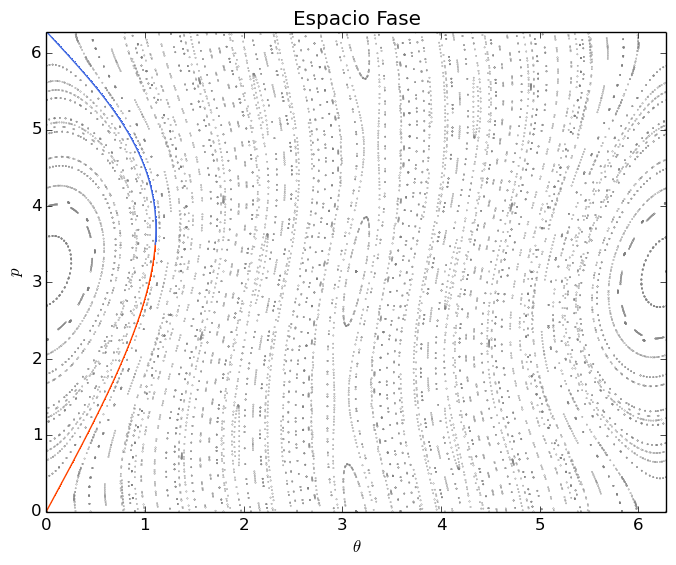
\includegraphics[scale=0.6]{estandark03}
 \caption{$W^{s},W^{u}$ de oden $25$ en el mapeo estándar con $\kappa=0.3$ y $t_{max}=3.0$.}
 \label{estandar03}
\end{figure}

\begin{figure}[H]
\centering
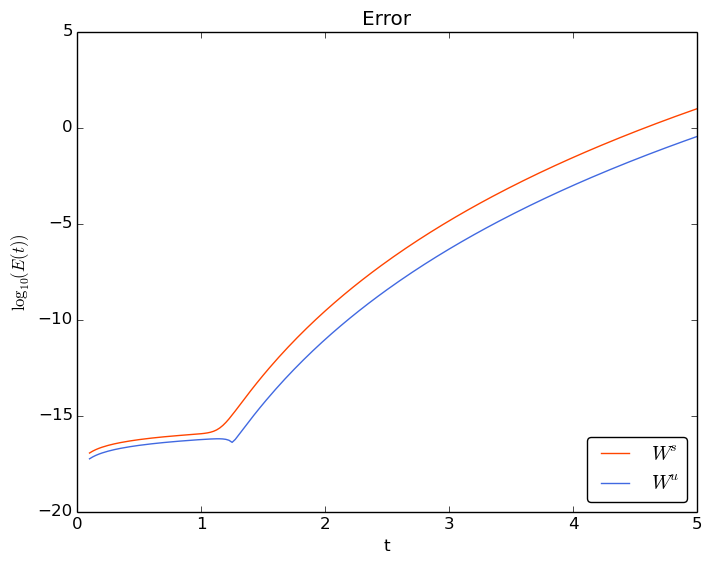
\includegraphics[scale=0.6]{error_est_k03} 
\caption{Error en las variedades de la figura \ref{estandar03}.}
\label{error est k03}
\end{figure}


\begin{figure}[H]
\centering
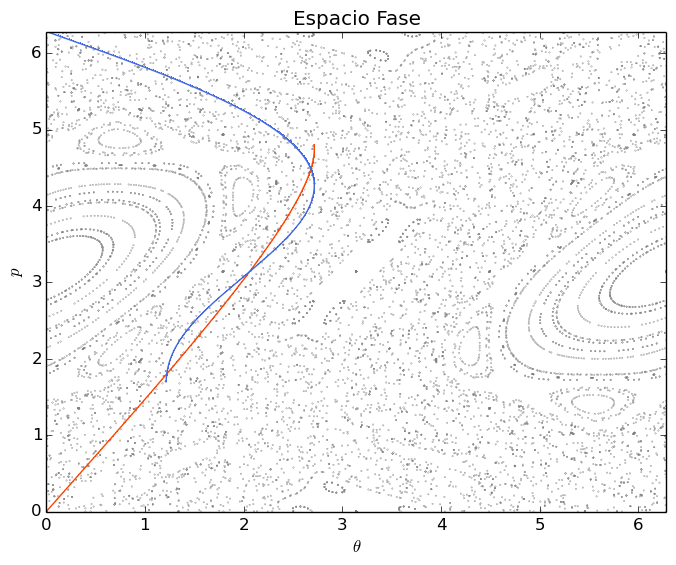
\includegraphics[scale=0.6]{estandark15}
\caption{$W^{s},W^{u}$ de orden $80$ en el mapeo estándar con $\kappa=1.5$ y $t_{max}=13.0$.}
\label{estandar15}
\end{figure}

\begin{figure}[H]
\centering
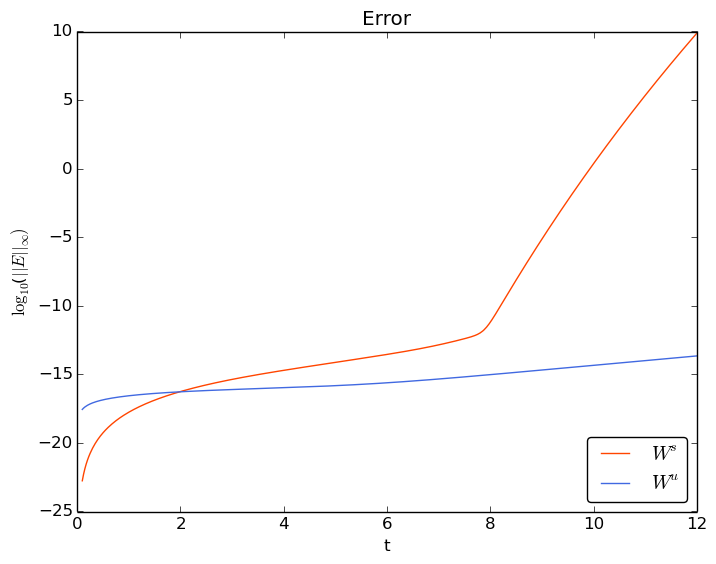
\includegraphics[scale=0.6]{error_est_k15} 
\caption{Error en las variedades de la figura \ref{estandar15}.}
\label{error est k15}
\end{figure}




\begin{figure}[H]
\centering
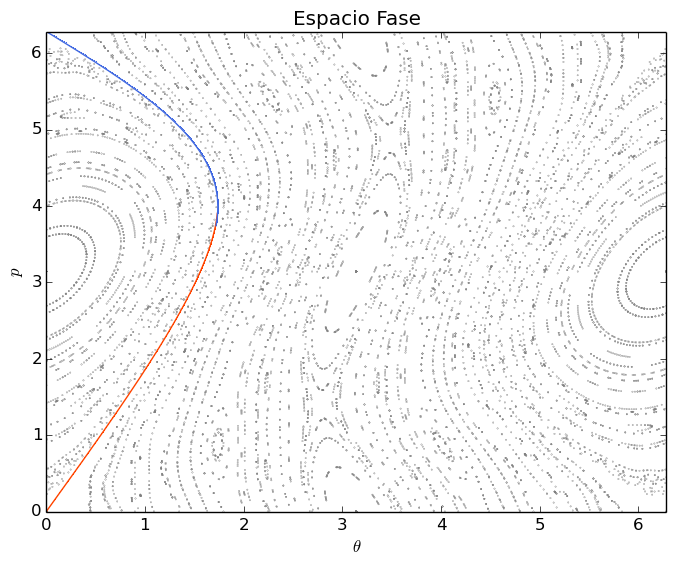
\includegraphics[scale=0.6]{estandark07}
\caption{$W^{s},W^{u}$ de orden 70 en el mapeo estándar con $\kappa=0.7$ y $t_{max}=5.5$.}
\label{estandar07}
\end{figure}

\begin{figure}[H]
\centering
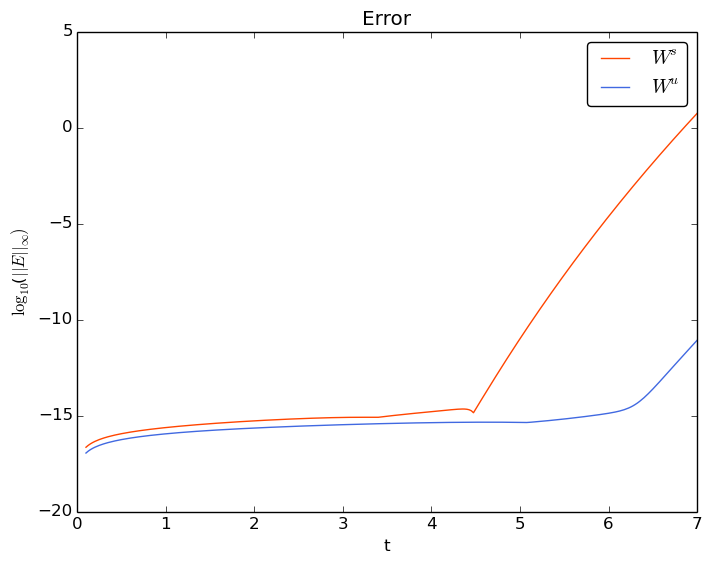
\includegraphics[scale=0.6]{error_est_k07} 
\caption{Error en las variedades de la figura \ref{estandar07}.}
\label{error est k07}
\end{figure}


En las figuras \ref{estandar03}-\ref{error est k07} se muestran los resultados de la parametrización de las variedades estable e inestable asociadas al punto fijo $\mathbf{x}=(0,0)$ para diferentes valores del parámetro $\kappa$, junto con cada una aparece su respectiva gráfica del error numérico.   Los cálculos se hicieron utilizando números de punto flotante de 64 bits(Float64). Para las figuras \ref{estandar03}, \ref{estandar07} se puede ver que las variedades se juntan de manera que parecen ser tangentes, mientras que para el caso de la figura \ref{estandar15} observamos varias intersecciones entre las variedades. En todos los casos el error se comporta de manera similar, manteniendose prácticamente constante hasta cierto valor del parámetro $t$ y creciendo de forma exponencial después del mismo. La curva será entonces confiable hasta valores del parámetro que no excedan el punto donde el error crece rápidamente.  \\


Para observar como cambiaba el comportamiento del error respecto del orden de la parametrización se calcularon polinomios de diferente orden que parametrizan a la variedad inestable del mapeo con $\kappa=0.3$,el resultado se muestra en la figura \ref{erroresf64}. Observamos que mientras más grande sea el orden del polinomio mejor es la aproximación, pues podemos llegar a valores del parámetro más grandes, que se traduce en ir más lejos en la variedad inestable. \\

\begin{figure}[H]
\centering
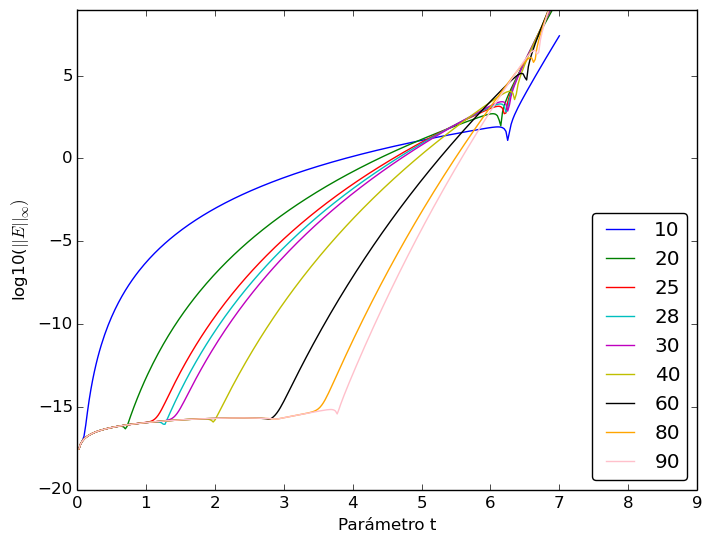
\includegraphics[scale=0.6]{error_estandar_orden}
\caption{Curvas de error para diferentes órdenes en el mapeo estándar,$\kappa=0.3$. }
\label{erroresf64}
\end{figure}
A fin de mostrar que el error es de alguna manera controlable se usaron números de presición extendida para hacer cálculos análogos a los anteriores. En la figura \ref{erroresBig} se muestran los resultados para parametrizaciones de ordenes entre $10$ y $80$. Observamos un comportamiento análogo, de tal manera que para cada orden diferente de parametrización hay un valor diferente del parámetro en el cuaĺ pasa de un error que no crece significativamente a un error que crece de manera abrupta. También notamos que al usar presición extendida el error cerca del punto fijo es imperceptible pero en la parte donde crece, tiene un crecimiento más pronunciado que en el caso de números de punto flotante. 

\begin{figure}[H]
\centering
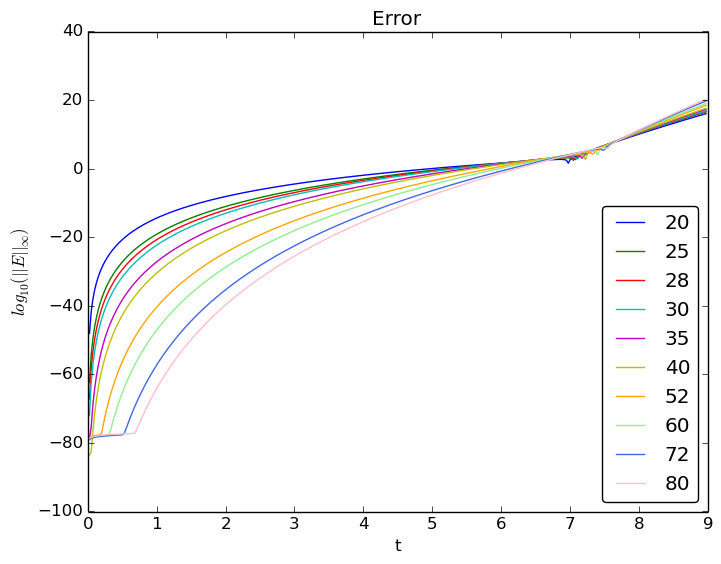
\includegraphics[scale=0.6]{error_estandar_orden_big}
\caption{Curvas de error para diferentes órdenes usando precisión extendida ,$\kappa=0.3$. }
\label{erroresBig}
\end{figure}

Como ya mencionamos antes la variedad inestable del mapeo inverso corresponde a la variedad estable del mapeo, por lo que si se usa el mismo método calculando la variedad inestable del mapeo inverso \ref{mapeo estandar inverso} podemos controlar mejor el error numérico. Para mostrar esto hicimos una comparación parametrizando la variedad estable mediante el mapeo inverso y el mapeo inicial. Los polinomios fueron del mismo orden y lo que se observó en el error se muestra en la figura \ref{erroresinverso}.


\begin{figure}[H]
\centering
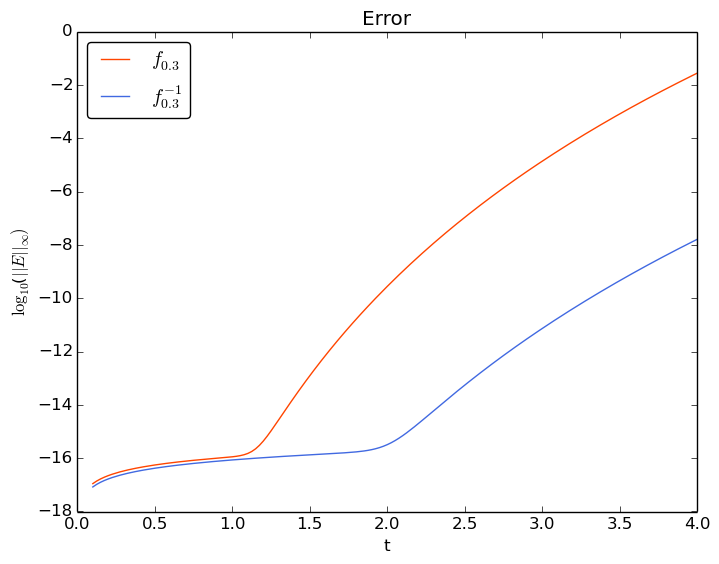
\includegraphics[scale=0.6]{mapeoinver}
\caption{Error para las parametrizaciones usando el mapeo y el mapeo inverso con polinomios de orden $20$ y $\kappa=0.3$. }
\label{erroresinverso}
\end{figure}




\section{Mapeo de Hénon}
El mapeo de Hénon se define como \cite{devaney}
\begin{eqnarray}
\mathbf{f}_{a,b}(x,y)=\left( \begin{array}{lcc}
             a-by-x^{2}\\
             \\ x
             \end{array}
             \right) \label{Henon}
\end{eqnarray}

siendo el mapeo inverso
\begin{eqnarray}
\mathbf{f}^{-1}_{a,b}(x,y)=\left( \begin{array}{lcc}
             y\\
             \\ (x+y^{2}-a)/-b
             \end{array}.
             \right) \label{HenonI}
\end{eqnarray} 

       
Para poder analizarlo debemos linearizar el sistema. Primero obtenemos el jacobiano 
            
\begin{eqnarray}
D\mathbf{f}_{a,b}(x,y)= \left( \begin{array}{lcc}
                -2x & -b\\
                \\ 1 & 0
                \end{array}
                \right)
\end{eqnarray}

                
Notamos que el determinante del jacobiano no es igual a uno sino $\det(D\mathbf{f}_{a,b}(x,y))=b$.
El determinante es constante, entonces será hamiltoniano en el caso en que $b$ sea igual a uno o menos uno. Analizaremos estos casos, primero encontrando los puntos fijos
\begin{eqnarray}
\mathbf{f}_{a,b}(x,y)=\left( \begin{array}{lcc}
               a-by-x^{2}\\
               \\ x
               \end{array}
               \right) = \left(\begin{array}{lc}
               x \\
               \\ y
               \end{array}
               \right)
\end{eqnarray}
              
lo que implica que $a-by-x^{2}=x$ y $x=y$ de donde es claro que la primer ecuación queda
\begin{eqnarray*}
x^{2}+(b+1)x-a=0
\end{eqnarray*}
que se puede resolver usando la fórmula general
\begin{eqnarray*}
x=\frac{-(b+1)\pm ((b+1)^{2}+4a)^{1/2} }{2}
\end{eqnarray*}
para el caso en que $b=1$ se tiene
\begin{eqnarray}
x=\frac{-2\pm 2(1+a)^{1/2} }{2}
\end{eqnarray}
Al escoger $b=1$ garantizamos estar en un sistema hamiltoniano, mientras que $a$ debe escogerse de manera que resulten puntos fijos hiperbólicos. La figura \ref{Henon1} muestra un ejemplo en cálculos de variedades para el mapeo de Hénon, junto con el error. 
\begin{figure}[H]
\centering
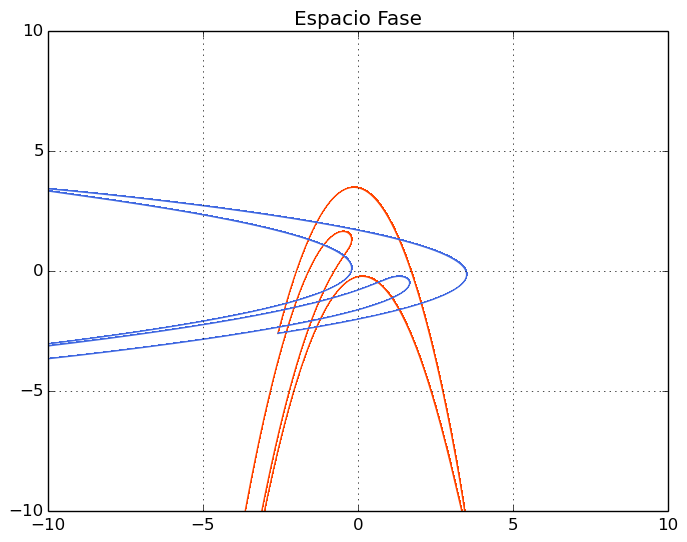
\includegraphics[scale=0.6]{henon1}
\caption{$W^{u}$ y $W^{s}$ de orden 45 con $t_{max}=1000.0$ para el mapeo de Hénon con $a=1.5$,$b=1$.}
\label{Henon1}
\end{figure}

\begin{figure}[H]
\centering
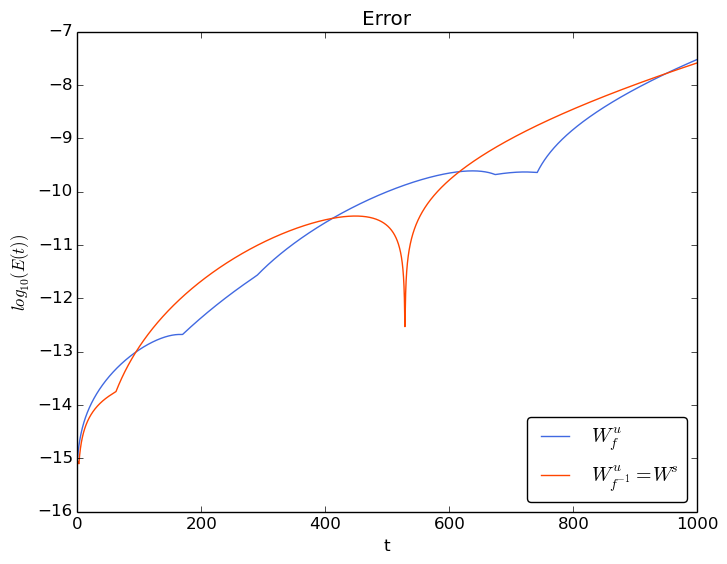
\includegraphics[scale=0.6]{ErrorHenon1}
\caption{Error asociado a las variedades de la figura \ref{Henon1}.}
\label{ErrorHenon1}
\end{figure}
Las variedades que aparecen en la figura \ref{Henon1} fueron calculadas con el mapeo de Hénon inicial \ref{Henon}, las variedades se observan simétricas, aún así las parametrizaciones son diferentes. Puede verse en el error, figura \ref{ErrorHenon1}, que la variedad estable tiene un mayor error que la variedad inestable, mientras en la inestable el error cambia cinco órdenes de magnitud, en todo el intervalo del parámetro, el error de la variedad estable cambia en al menos quince órdenes de magnitud. \\

A diferencia del mapeo estándar en éste mapeo las órbitas pueden irse al infinito, es decir no están  constreñidas en una sección fija, lo que representa un mayor reto en cuanto a la parametrización ya que el polinomio debe ser tal que pueda regresar varias veces. De hecho podemos observar que se necesitan valores realmente grandes, comparados con los del mapeo estándar, para observar los cruces de las variedades. También esta situación hace que el error numérico sea mayor que para el estándar. \\

En las figuras \ref{Henon2}, \ref{Henon3} se muestran las variedades calculadas de la misma manera en la que se calcularon para la figura \ref{Henon1}. En \ref{Henon2} las curvas son más cerradas y se necesita de un polinomio de orden mayor que en el caso de \ref{Henon3} para observar los cortes. 
\begin{figure}[H]
\centering
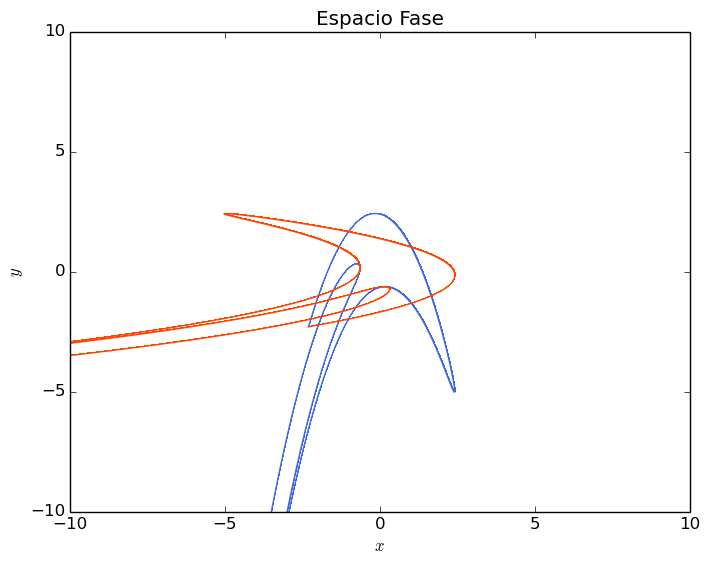
\includegraphics[scale=0.6]{henon2}
\caption{$W^{u}$, $W^{s}$ de orden $50$ y $t_{max}=800.0$ para el mapeo de Hénon con $a=0.7$,$b=1.$.}
\label{Henon2}
\end{figure}

\begin{figure}[H]
\centering
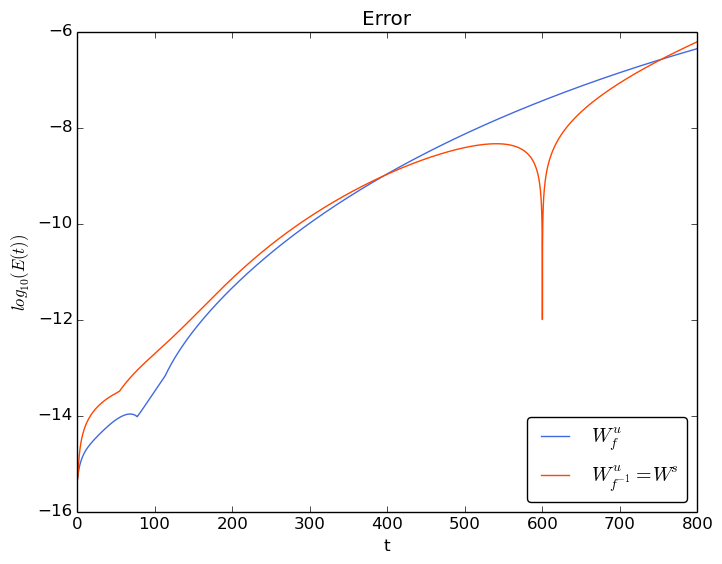
\includegraphics[scale=0.6]{ErrorHenon2}
\caption{Error asociado a las variedades de la figura \ref{Henon2}.}
\label{Henon2}
\end{figure}


\begin{figure}[H]
\centering
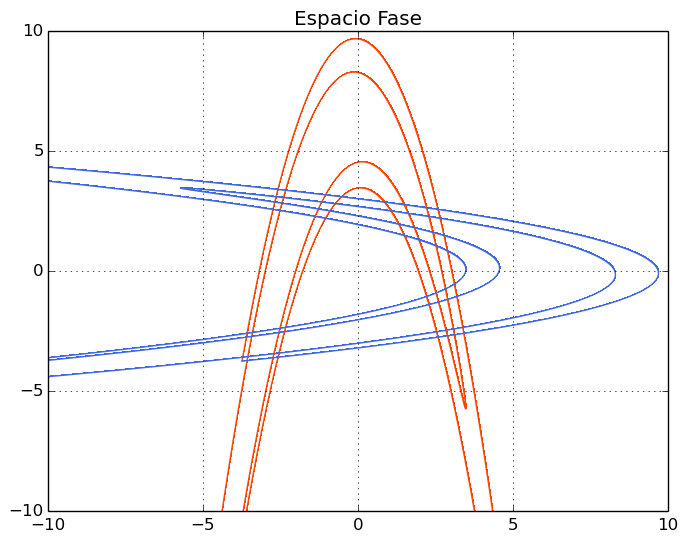
\includegraphics[scale=0.6]{henon3}
\caption{$W^{u}$, $W^{s}$ de orden $78$ y $t_{max}=4000.0$ para el mapeo de Hénon con $a=6.5$,$b=1.$.}
\label{Henon3}
\end{figure}

\begin{figure}[H]
\centering
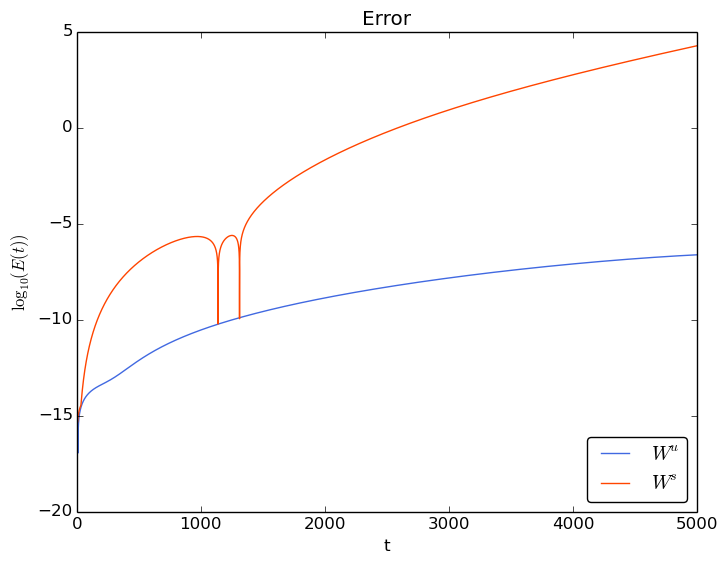
\includegraphics[scale=0.6]{ErrorHenon3}
\caption{Error asociado a las variedades de la figura \ref{Henon3}.}
\label{Henon3}
\end{figure}


Asi que con el orden suficiente es posible observar los cruces de ambas variedades, retomaremos esto en la última sección. 

\section{Mapeo exponencial}
El último mapeo que se estudió fue uno presentado en el artículo \citep{Jung} el cual queda definido por 
\begin{eqnarray}
\mathbf{j}_{a}(x,y)=\left(\begin{array}{lcc}
             x+y\\
             \\ y+af(x+y)
             \end{array}\right)
\label{Jung}
\end{eqnarray}

que describe el movimiento de una partícula pateada , donde la coordenada $x$ representa la posición en una dimensión mientras que la coordenada $y$ es el momento, $a$ es un parámetro libre. La función $f$ es la responsable de describir la fuerza aplicada, en el artículo \cite{Jung} se escoge
\begin{eqnarray*}
f(x)=x(x-1)e^{-x}.
\end{eqnarray*}
Al cual le corresponde su inverso
\begin{eqnarray}
\mathbf{j}^{-1}_{a}(x,y)=\left(\begin{array}{lcc}
             x-y+ax(x-1)e^{-x}\\
             \\ y-ax(x-1)e^{-x}
             \end{array}\right).
             \label{jungI}
\end{eqnarray}
En este sistema los puntos fijos encontrados son $x_{0}=(1,0),x_{1}=(0,0)$ donde $x_{0}$ es un punto fijo hiperbólico. El punto $x_{1}$ es un punto elíptico mientras el valor del parámetro sea menor a 4, para valores de $a \geq 4$ se torna inverso hiperbólico.\\

Aplicando el mismo mecanismo que en los casos pasados se obtuvieron las figuras \ref{jung1}-\ref{errorjung2} que muestran cómo se comportan las variedades aún en el caso en que el sistema no sea completamente hiperbólico. Como en los casos anteriores el error asociado a la variedad estable es mayor que el asociado a la inestable. Al parecer la forma exponencial del mapeo también hace que el error crezca de manera exponencial para la estable. El orden al que se debe llegar en los polinomios para observar algunos de los cortes de las variedades es más alto en comparación con el mapeo de Hénon debido a que en este caso se esta aproximando una función exponencial.

\begin{figure}[H]
\centering
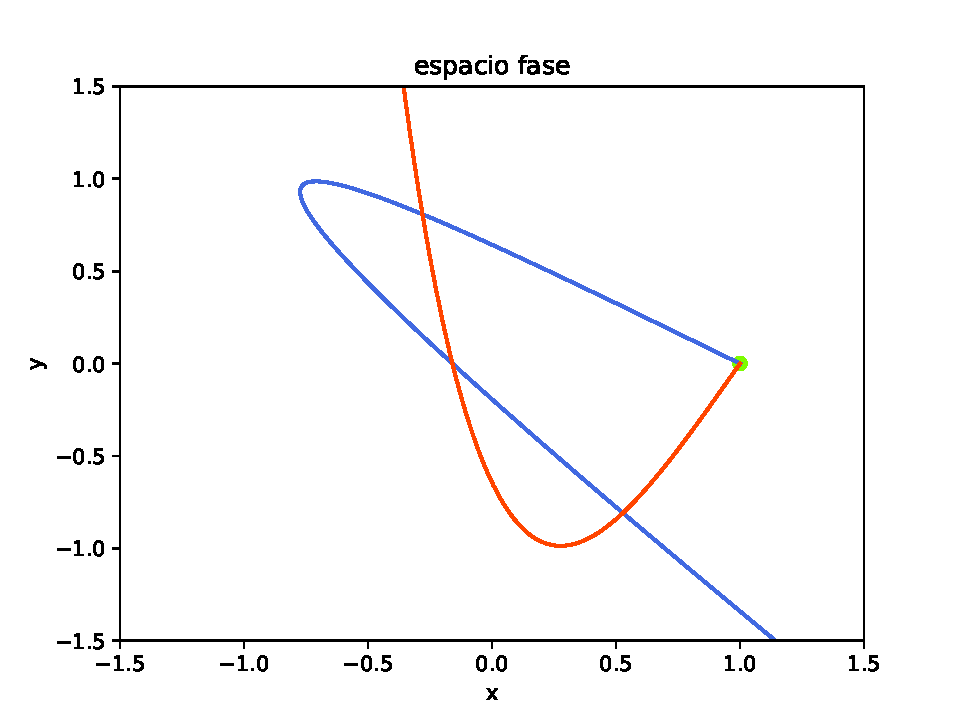
\includegraphics[scale=0.6]{jung34}
\caption{$W^{s}$ de orden 93, $W^{u}$ de orden 86 con $t_{max}=5.5$, con $a=3.4$ en el punto fijo $x_{0}$.}
\label{jung1}
\end{figure}


\begin{figure}[H]
\centering
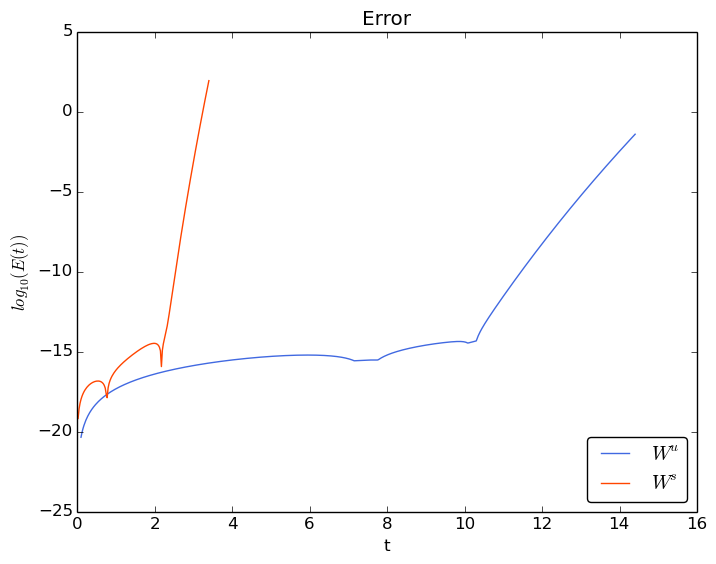
\includegraphics[scale=0.6]{error_jung34}
\caption{Error asociado a las variedades de la figura \ref{jung1}.}
\label{errorjung1}
\end{figure}




\begin{figure}[H]
\centering
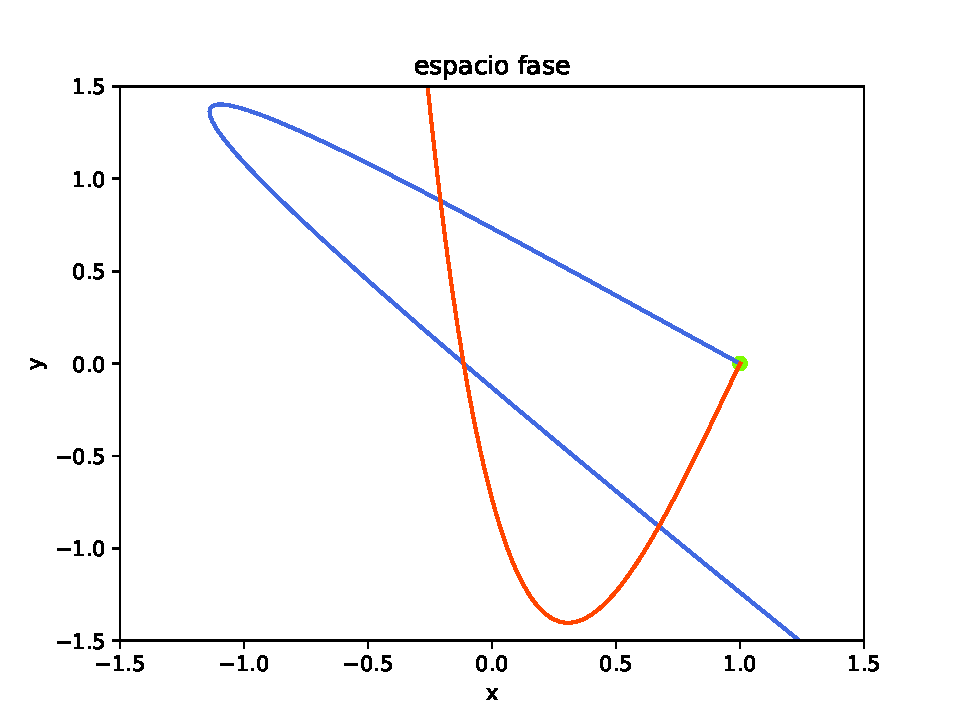
\includegraphics[scale=0.6]{jung57}
\caption{$W^{s}$ de orden 90, $W^{u}$ de orden 87 con $t_{max}=6.5$, con $a=5.7$ en el punto fijo $x_{0}$.}
\label{jung2}
\end{figure}


\begin{figure}[H]
\centering
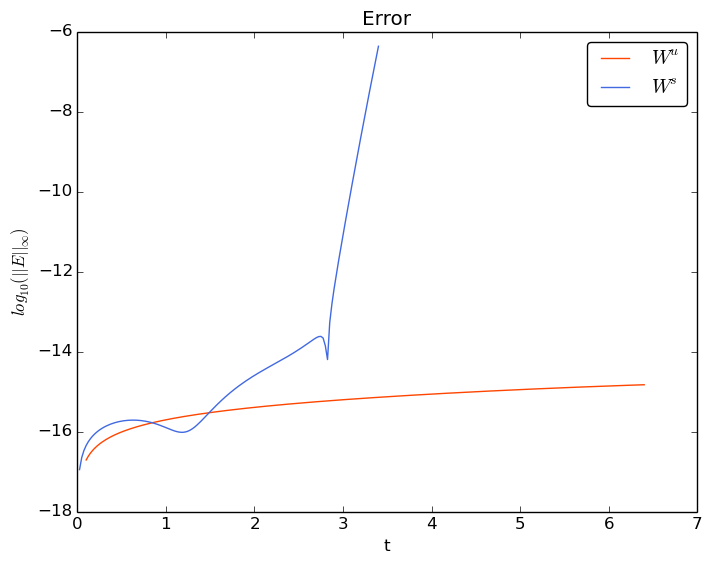
\includegraphics[scale=0.6]{error_jung57}
\caption{Error asociado las variedades de la figura \ref{jung2}}
\label{errorjung2}
\end{figure}


\section{Convergencia}
Además de medir el error asociado a la parametrización consideramos importante tomar en cuenta la convergencia de los coeficientes de los polinomios. En casos como el mapeo exponencial en que las variedades se acercan a puntos fijos de diferente naturaleza puede ocurrir que tal cercanía afecte la forma de parametrización. Para ello se implementaron dos formas de revisar la convergencia, la de Hadamard \ref{hadamard} y la de tres términos \ref{tres terminos}. \\

La figura \ref{convergenciaEst15} muestra la convergencia de los polinomios de orden 25 que parametrizan la variable $\theta$ en el mapeo estádar para las variedades estable e inestable con $\kappa=1.5$ a la que correponde el espacio fase mostrado en \ref{estandar15}. En el caso de la variedad estable se ve que los coeficientes cambian de manera abrupta al principio pero después de cierta $n$ el cociente es casi cero. Para el caso de la variedad inestable los coeficientes cambian de manera suave y el cociente también se acerca a cero. En ambos casos podemos decir que los coeficientes de la parametrización convergen a cero.  
\begin{figure}[H]
\centering
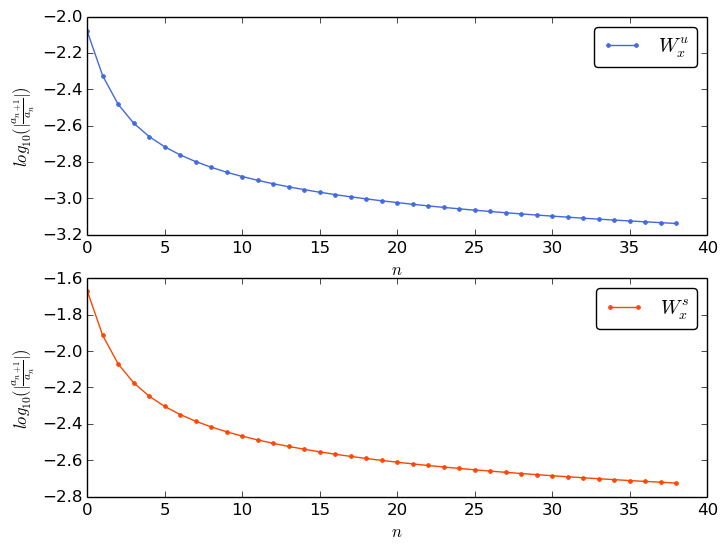
\includegraphics[scale=0.5]{converEst15}
\caption{Convergencia de Hadamard asociada a los polinomios para $\theta$ en las variedades del mapeo estándar con $\kappa=1.5$}
\label{convergenciaEst15}
\end{figure}

La figura \ref{convergenciaHenon1} muestra la convergencia de las parametrizaciones de orden 45 para la variable $x$ en el mapeo de Hénon con $a=1.5$. En ambos casos la convergencia parece suave y tiende a cero y igual que en el caso del mapeo estándar.

\begin{figure}[H]
\centering
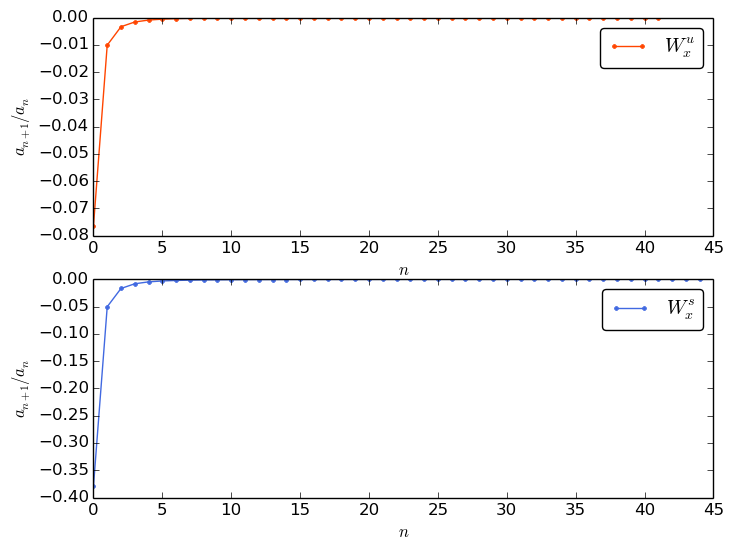
\includegraphics[scale=0.5]{converHenon1}
\caption{Convergencia de Hadamard asociada a los polinomios para $x$ en las variedades del mapeo de Hénon con $a=1.5$}
\label{convergenciaHenon1}
\end{figure}


Para el mapeo exponencial realizamos los dos criterios de convergencia. La figura \ref{convergenciaJH} muestra el criterio de Hadamard \ref{hadamard} para los polinomios que parametrizan la variable x en cada variedad, se ve que hay una convergencia clara de ls coeficientes. Lo mismo ocurre en la figura \ref{convergenciaJ3} en dónde se usó el criterio de tres términos \ref{tres terminos}.

\begin{figure}[H]
\centering
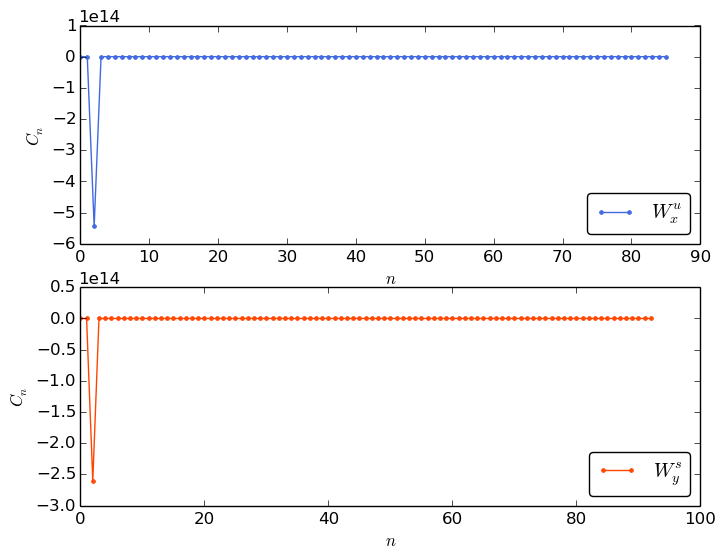
\includegraphics[scale=0.5]{convergenciaJungH57}
\caption{Convergencia de Hadamard asociada a las variedades mostradas en la figura \ref{jung2}.}
\label{convergenciaJH}
\end{figure}


\begin{figure}[H]
\centering
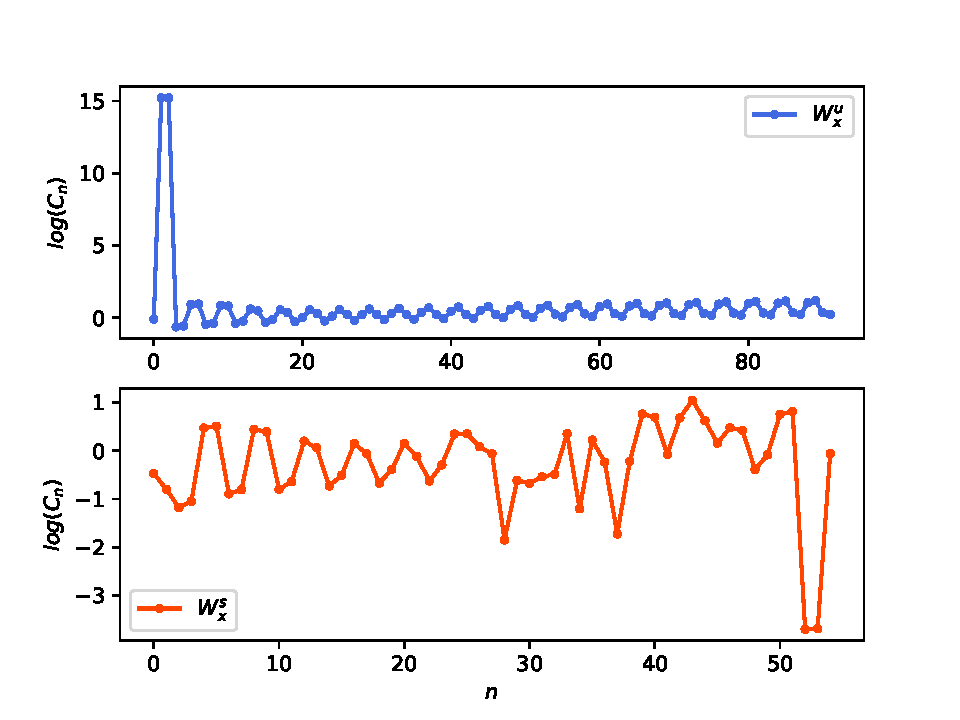
\includegraphics[scale=0.5]{convergenciaJungT57}
\caption{Convergencia de tres términos asociada a las variedades en la figura \ref{jung2}}
\label{convergenciaJ3}
\end{figure}

Estudiar la convergencia de las parametrizaciones puede dar una idea de cómo se va modificando el polinomio si se cambia el orden, en mapeos más sensibles puede ser determinante para saber en a qué orden es conveniente aproximar. 

\section{Existencia de puntos homoclínicos}

Siendo que el resultado son polinomios se puede aplicar el método de Newton en dos dimensiones o cualquier otro para resolver $P^{u}=P^{s}$ y encontrar puntos homoclínicos o heteroclínicos. Por suerte existe una paquetería en Julia que hace cálculos númericos validados \texttt{ValidatedNumerics}\cite{validated} dentro de la cuál se tiene un paquete para aritmética de intervalos \texttt{IntervalArithmetic}\citep{interval} y para encontrar raíces \texttt{IntervalRootFinding}\cite{root} además del paquete \texttt{Static Arrays}\cite{static} que permite manipular intervalos.\\ 

El paquete \cite{validated} hace cálculos de computación rigurosa con números de punto flotante usando el paquete de aritmética de intervalos, que efectúa operaciones con intervalos en lugar de números. Mientras que \cite{root} automatiza el métodos populares como el de Newton para encontrar raíces de funciones, en este caso se garantiza que la respuesta correcta se encuentra en un intervalo. Para entender méjor cómo funcionan cada una de las paqueterías así como la teoría rigurosa detrás de éstos recomendamos revisar las lecturas \cite{ramon},\cite{Numerics}. 

En forma simple si $[a,b],[c,d]$ son intervalos en $\mathbb{R}$ entonces es posible definir las operaciones básicas, por ejemplo la suma $+$
\begin{eqnarray}
[a,b]+[c,d]=[a+b,c+d]
\end{eqnarray}
resulta bastante simple e intuitiva; la definición de otras operaciones puede verse en \ref{ramon}. La finalidad en nuestro caso de usar intervalos $[a,b]$ en lugar de un valor $x$ es que al encontrar un intervalo podemos afirmar que en tal se encuentra la raíz, sin embargo al calcular la raíz como un valor debemos tomar en cuenta que puede que ese valor no sea el exacto. Es decir debido a procesos de redondeo, así como de errores en la interpretación de un número real de manera computacional puede que nuestro valor de la raíz calculado de manera convencional no sea el valor correcto. Sin embargo al hacer aritmética de intervalos no encontramos la raíz en sí , encontramos un intervalo en donde podemos garantizar que se encuentra la raíz verdadera. Los métodos usados para calcular raíces con intervalos se valen de la generalización del método de Newton.

Para nuestro caso resulta que el programa arroja dos polinomios asociados a cada variedad, si definimos 
\begin{eqnarray}
P:=P^{u}(t)-P^{s}(t')=0
\label{CorteV}
\end{eqnarray}
podemos encontrar las intersecciones en un intervalo de 2 dimensiones que será $[a,b]\times[c,d]$ con $a,b,c,d \in \mathbb{R}$. 


\subsection{Estándar}

Usando esto en el mapeo stándar con una tolerancia de $10^{-5}$ se encontraron la siguientes intersecciones para un caso específico.
\begin{figure}[H]
\centering
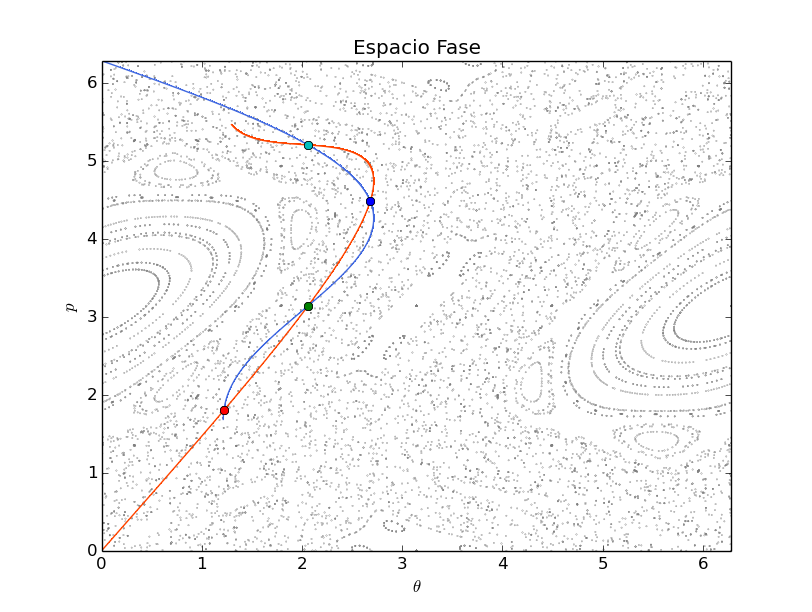
\includegraphics[scale=0.4]{cruce_estandar}
\caption{Cruces de $W^{u},W^{s}$ para el mapeo estándar con $k=1.5$ }
\label{cruce_estandar}
\end{figure}







\subsection{Hénon}
Como mencionamos en el mapeo estándar usando el paquete de aritmética de intervalos se pueden calcular las intersecciones de las variedades estable e inestable. En este caso para el mapeo de Hénon, donde el parámetro $a=1.5$ con un polinomio de orden 45, se usó el método con una tolerancia de $10^{-6}$ además de usar el mapeo inverso \ref{HenonI}, para calcular la variedad estable. 
 
Lo que resultó de resolver \ref{CorteV} fueron los siguientes intervalos:
\begin{itemize}
\item[a)] Root$([-1.36597, -1.36596] \times [166.749, 166.75]$, :unique)
\item[b)] Root$([-5.26555, -5.26554] \times [129.577, 129.578]$, :unique)
\item[c)] Root$([-6.77613, -6.77612] \times [33.6142, 33.6143]$, :unique)
\item[d)] Root$([-5.54438e-07, 0] \times [0, 5.54438e-07]$, :unknown)     
\item[e)] Root$([-26.1208, -26.1207] \times [26.1207, 26.1208]$, :unique)  
\item[f)] Root$([-33.6143, -33.6142] \times [6.77612, 6.77613]$, :unique)  
\item[g)] Root$([-129.578, -129.577] \times [5.26554, 5.26555]$, :unique) 
\item[h)] Root$([-166.75, -166.749] \times [1.36596, 1.36597]4$, :unique)
\end{itemize}

La leyenda \texttt{unique} concluye que hay una raíz en el intervalo y es única, mientras que \texttt{unknown} nos dice que no puede concliur si hay una o más. Si notamos el tercer intervalo contiene al cero $(t,t')=(0,0)$ en el cual se cortan las variedades pues representa el punto fijo. Para los intervalos encontrados se hizo una gráfica que representa el intervalo donde se encuentra el cruce. 


\begin{figure}[H]
\centering
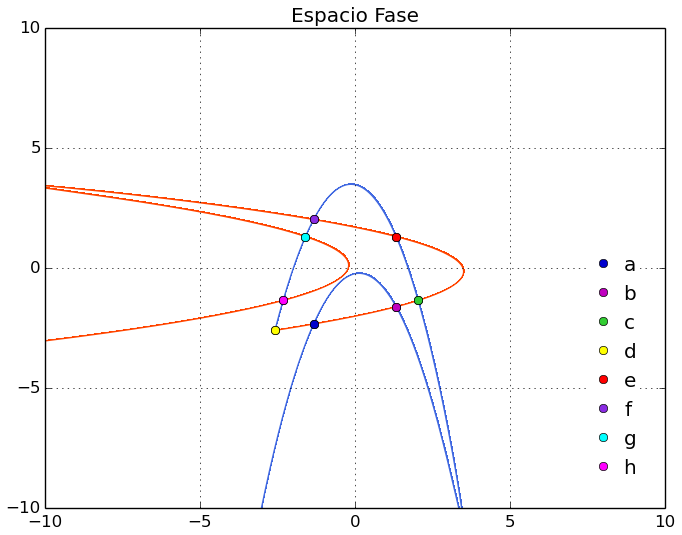
\includegraphics[scale=0.5]{crucesL}
\caption{Cruces de $W^{u},W^{s}$ encontrados en el intervalo $[-400.,0.] \times [0.,400.]$ }
\label{cruces}
\end{figure}

Donde cada punto indica un cruce econtrado, el punto de color es sólo para indicar cuaĺes fueron encontradas. En cuanto a el intervalo real en donde se encontró la intersección podemos encontrar las siguientes gráficas.


\begin{figure}[H]
\centering
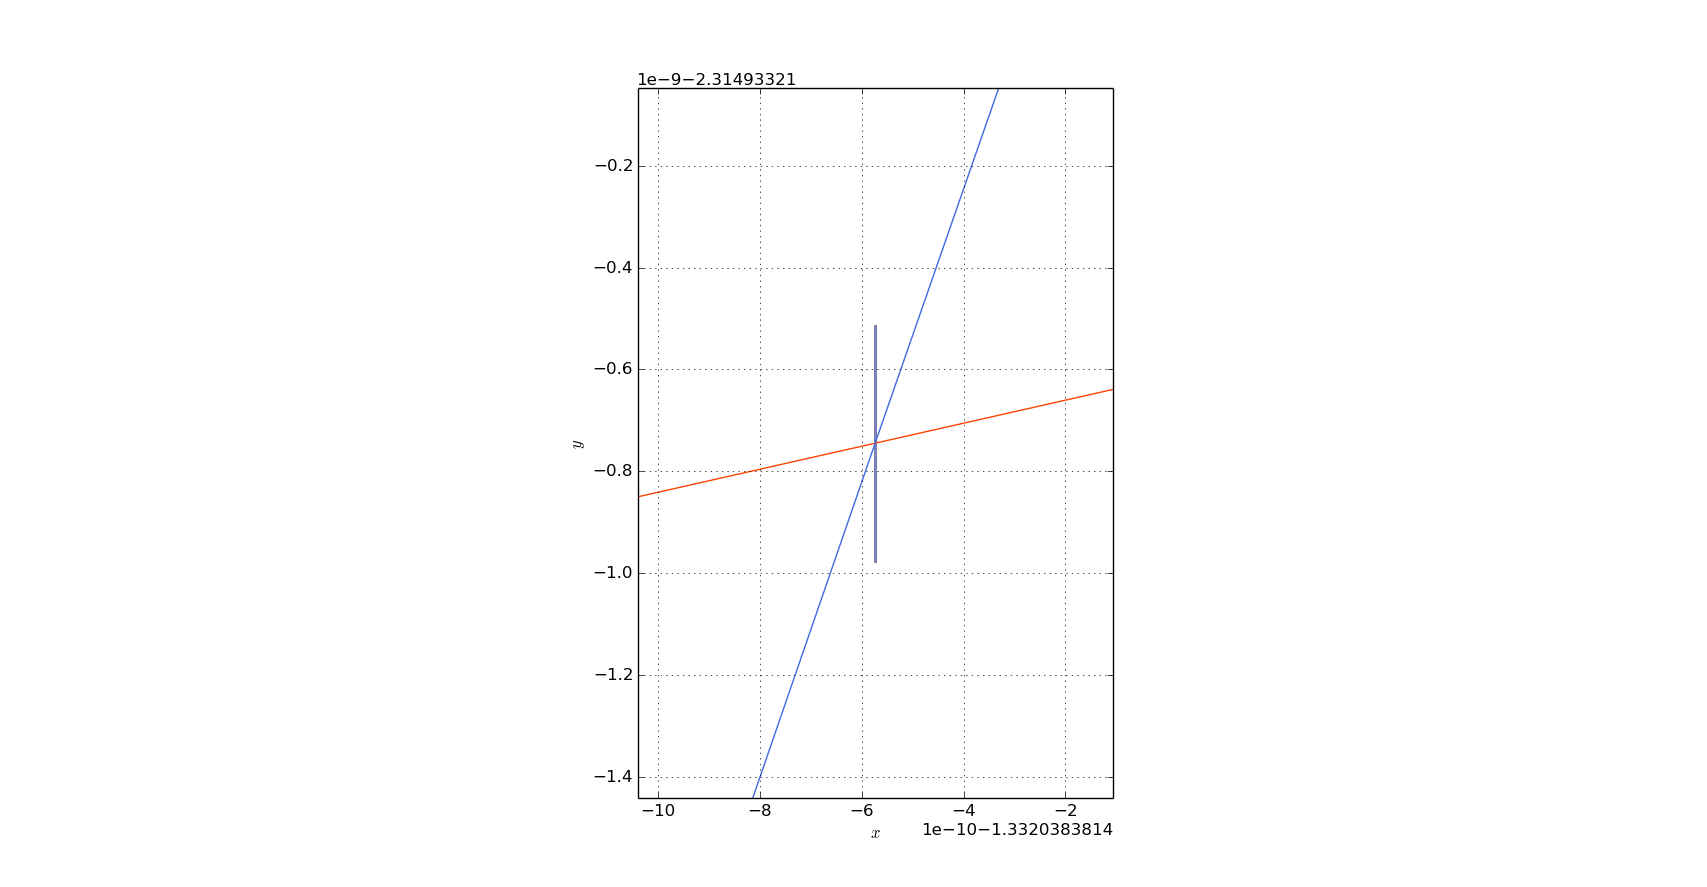
\includegraphics[scale=0.4]{cruce1}
\caption{Cruce de $W^{u},W^{s}$ encontrado con el intervalo a}
\label{cruce1}
\end{figure}

\begin{figure}[H]
\centering
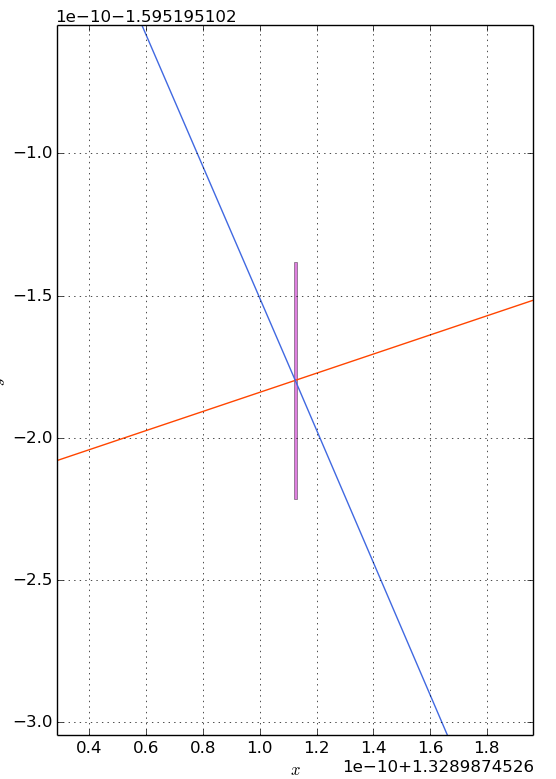
\includegraphics[scale=0.4]{cruce2}
\caption{Cruce de $W^{u},W^{s}$ encontrado con el intervalo b}
\label{cruce2}
\end{figure}


\begin{figure}[H]
\centering
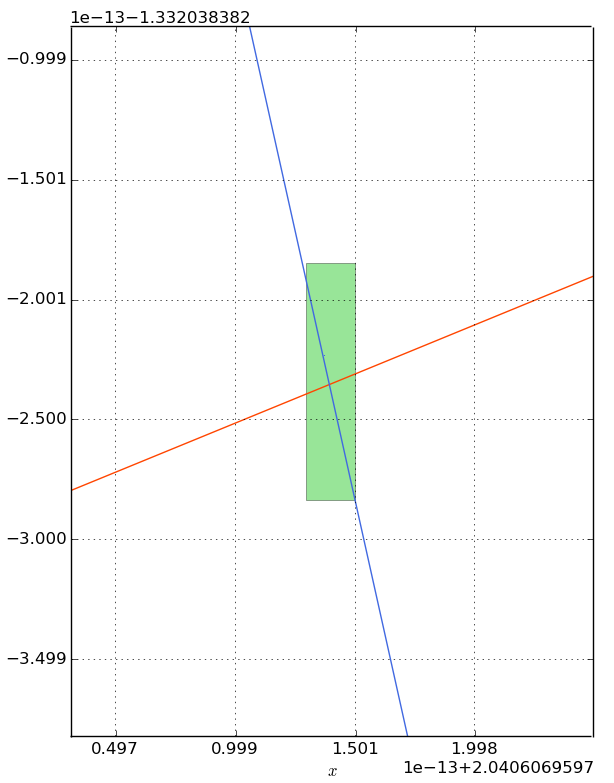
\includegraphics[scale=0.4]{cruce3}
\caption{Cruce de $W^{u},W^{s}$ encontrado con el intervalo c }
\label{cruce3}
\end{figure}


\begin{figure}[H]
\centering
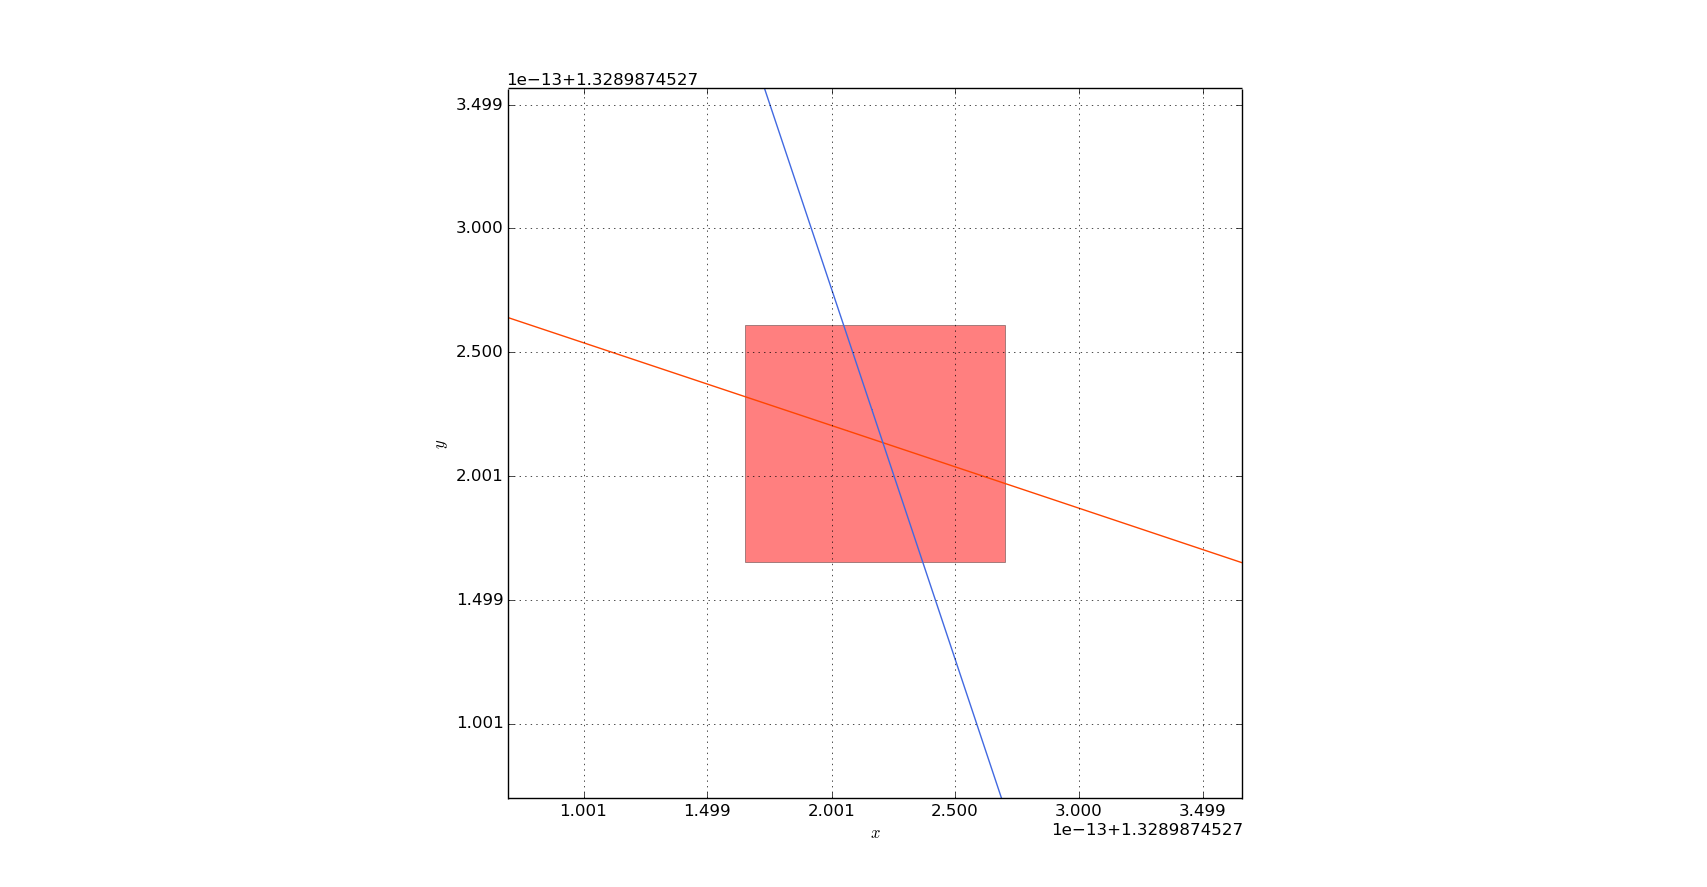
\includegraphics[scale=0.4]{cruce5}
\caption{Cruce de $W^{u},W^{s}$ encontrado con el intervalo e }
\label{cruce5}
\end{figure}

\begin{figure}[H]
\centering
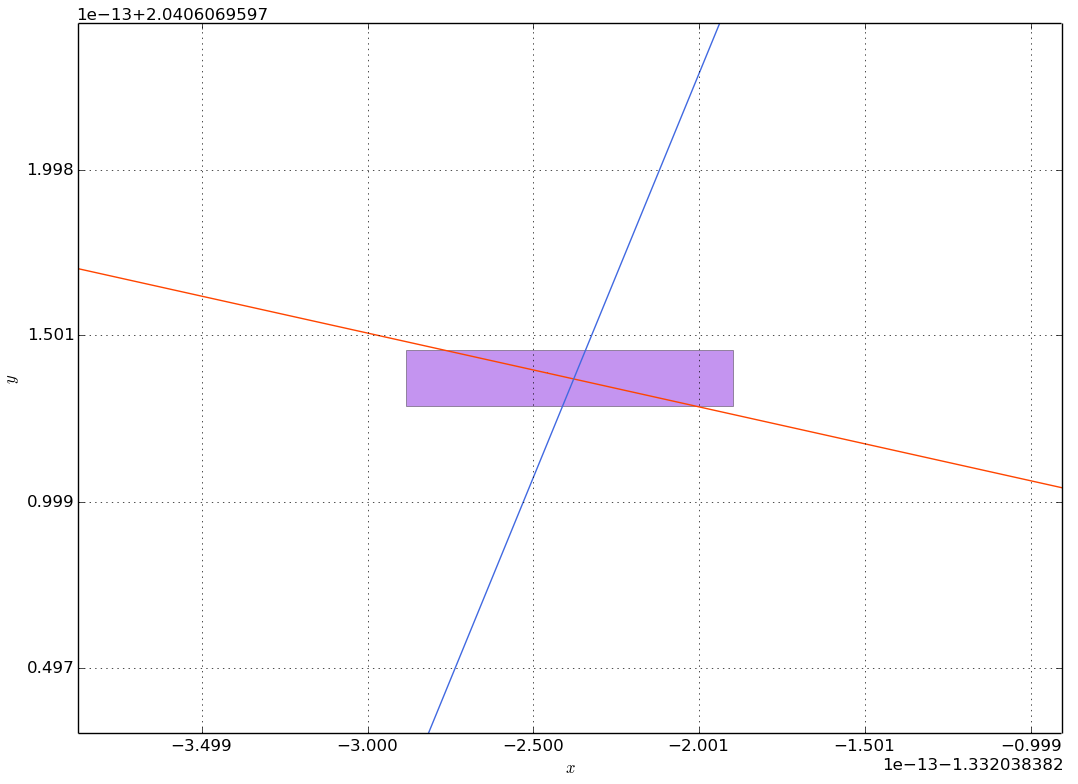
\includegraphics[scale=0.4]{cruce6}
\caption{Cruce de $W^{u},W^{s}$ encontrado con el intervalo f }
\label{cruce6}
\end{figure}

\begin{figure}[H]
\centering
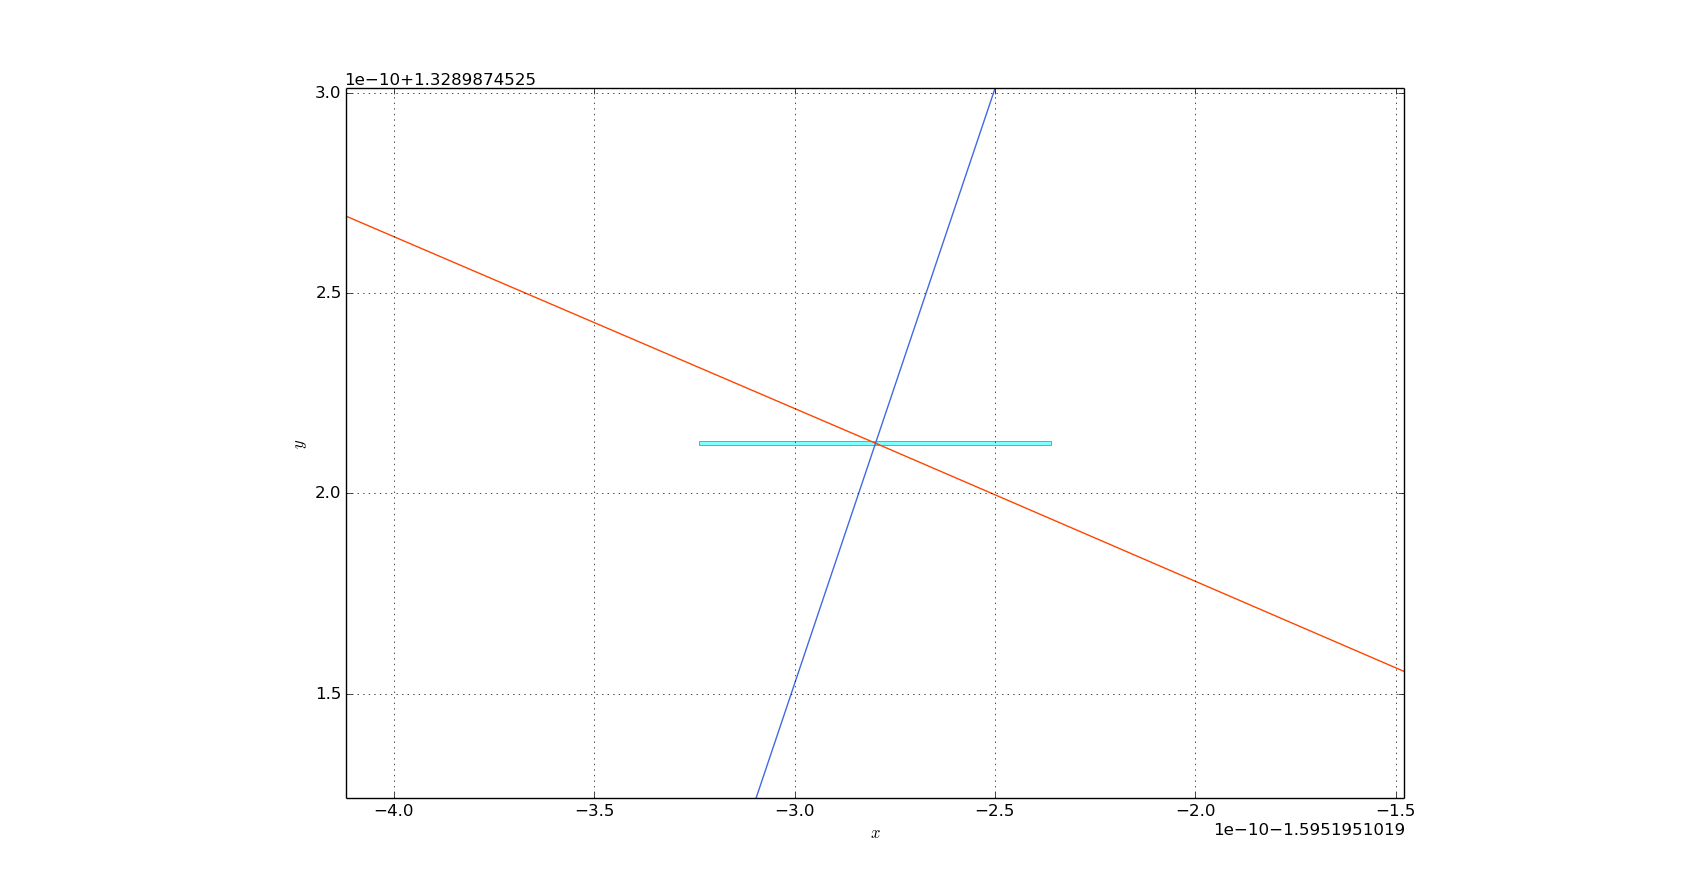
\includegraphics[scale=0.4]{cruce7}
\caption{Cruce de $W^{u},W^{s}$ encontrado con el intervalo g }
\label{cruce7}
\end{figure}

\begin{figure}[H]
\centering
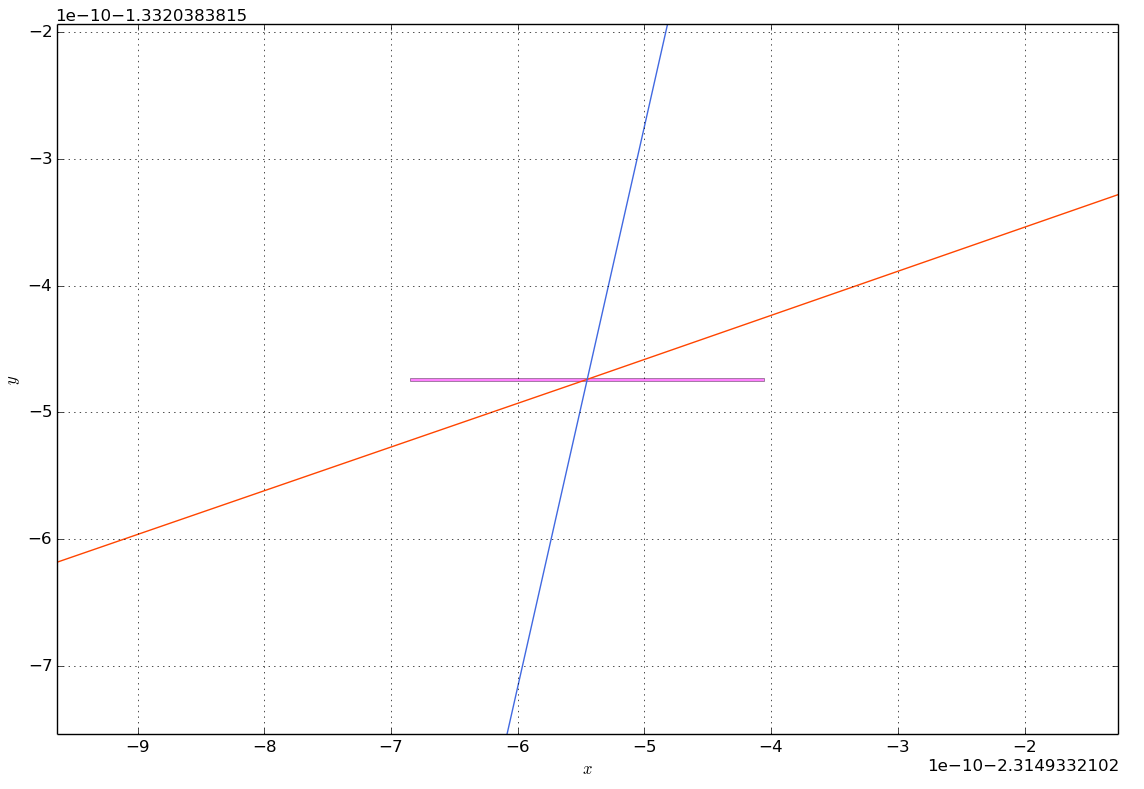
\includegraphics[scale=0.4]{cruce8}
\caption{Cruce de $W^{u},W^{s}$ encontrado con el intervalo h }
\label{cruce8}
\end{figure}


La zona rectangular sombreada en cada gráfica representa el producto cruz de los intervalos donde se encuentra la solución. Podemos observar que de hecho cada zona contiene el cruce de las variedades. Garantizando así que en el intervalo propuesto hay un cruce de variedades. Este tipo de resultados son útiles para hablar sobre caos. Hay que aclarar que los intervalos en los que se encuentra la intersección son intervalos en términos de los parámetros, no de las coordenadas del espacio fase, sin embargo conociendo cómo se mapean los intervalos en cada variedad podemos definir un nuevo intervalo en el espacio fase. \\


Para complementar todo este análisis se puede obtener una gráfica de las superficies que forman las variedades al cambiar el parámetro del mapeo lo que nos da una idea de como se ven las superficies y además de como se comportan las intersecciones. Las gráficas correspondientes a esto se encuentran en el sitio \textbf{LIGA}.
\subsection{Mapeo exponencial}
Además se analizaron los cruces en las variedades , usando como en los casos anteriores el mapeo inverso \ref{jungI}. Este mapeo representa un mayor reto en cuanto al orden del polinomio, la presencia de la exponencial hace que la parametrización sea sensible al orden del polinomio. Para el siguiente ejemplo se necesitó un polinomio de orden 86, en el cual se podía observar un comportamiento interesante, y se calcularon los cruces de las variedades como en los otros casos. 



\begin{figure}[H]
\centering
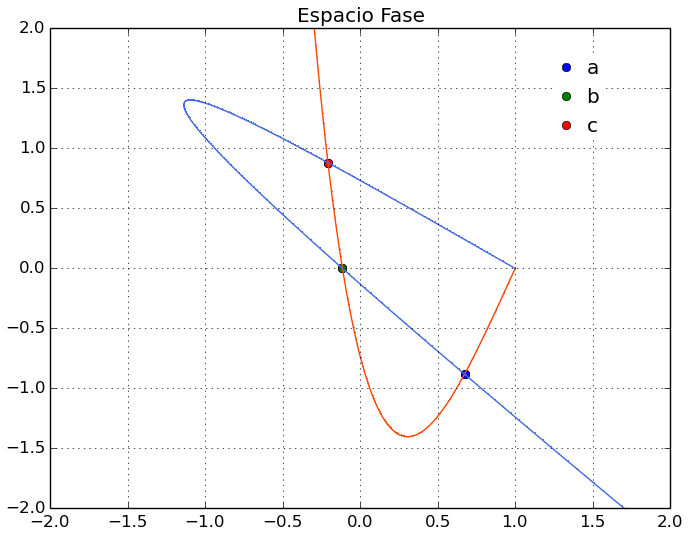
\includegraphics[scale=0.5]{cruces_jung1}
\caption{Intersecciones en el mapeo exponencial con $a=5.7$}
\label{jung_cortes}
\end{figure}
\begin{itemize}
\item[a)] Root$([-0.985068, -0.985067] \times [5.99488, 5.99489]$, :unique)
\item[b)] Root$([-3.46215, -3.46214] \times [5.49229, 5.4923]$, :unique)
\item[c)] Root$([-3.77896, -3.77895] \times [1.56269, 1.5627]$, :unique)
\end{itemize}
Tomando los cruces a escala del intervalo resultan las siguientes gráficas.

\begin{figure}[H]
\centering
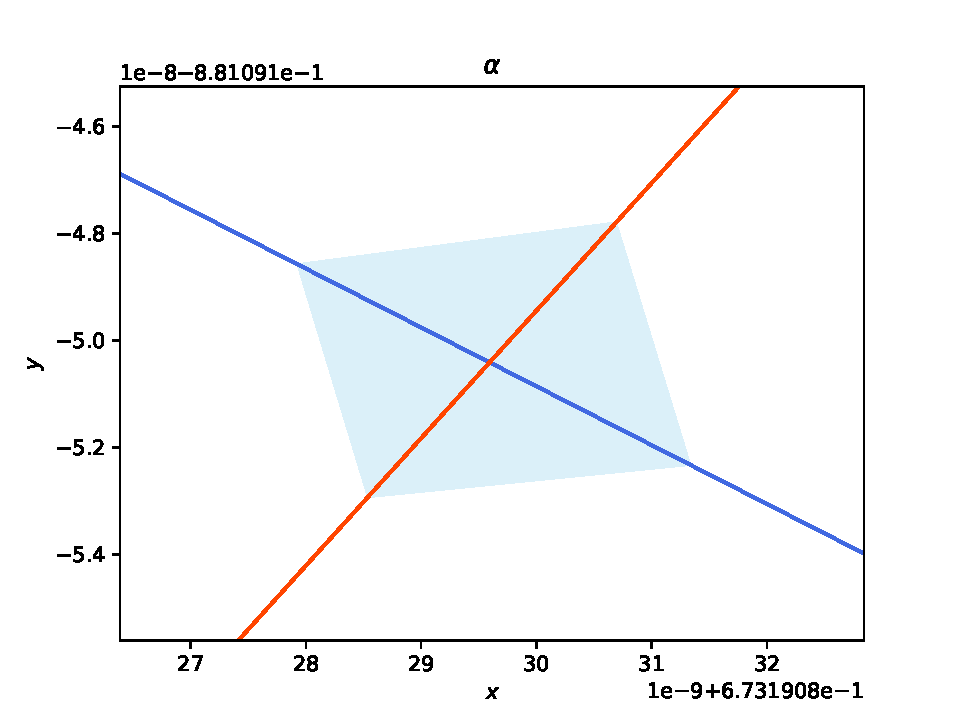
\includegraphics[scale=0.4]{cruce_a}
\caption{Intersección en el intervalo a}
\label{jung_corte1}
\end{figure}


\begin{figure}[H]
\centering
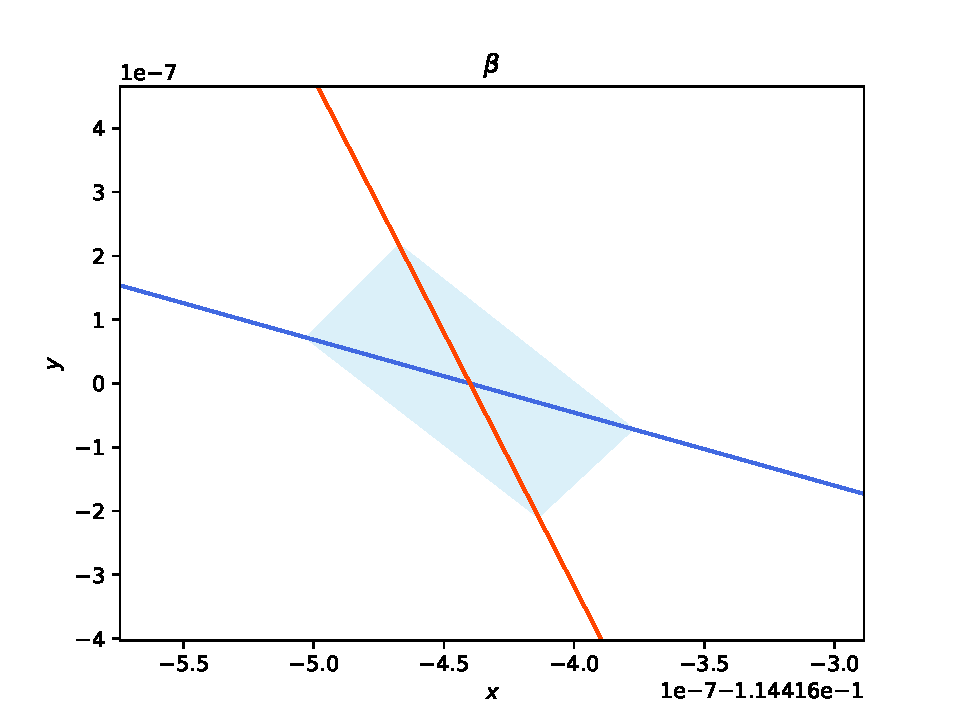
\includegraphics[scale=0.4]{cruce_b}
\caption{Intersección en el intervalo b}
\label{jung_corte2}
\end{figure}


\begin{figure}[H]
\centering
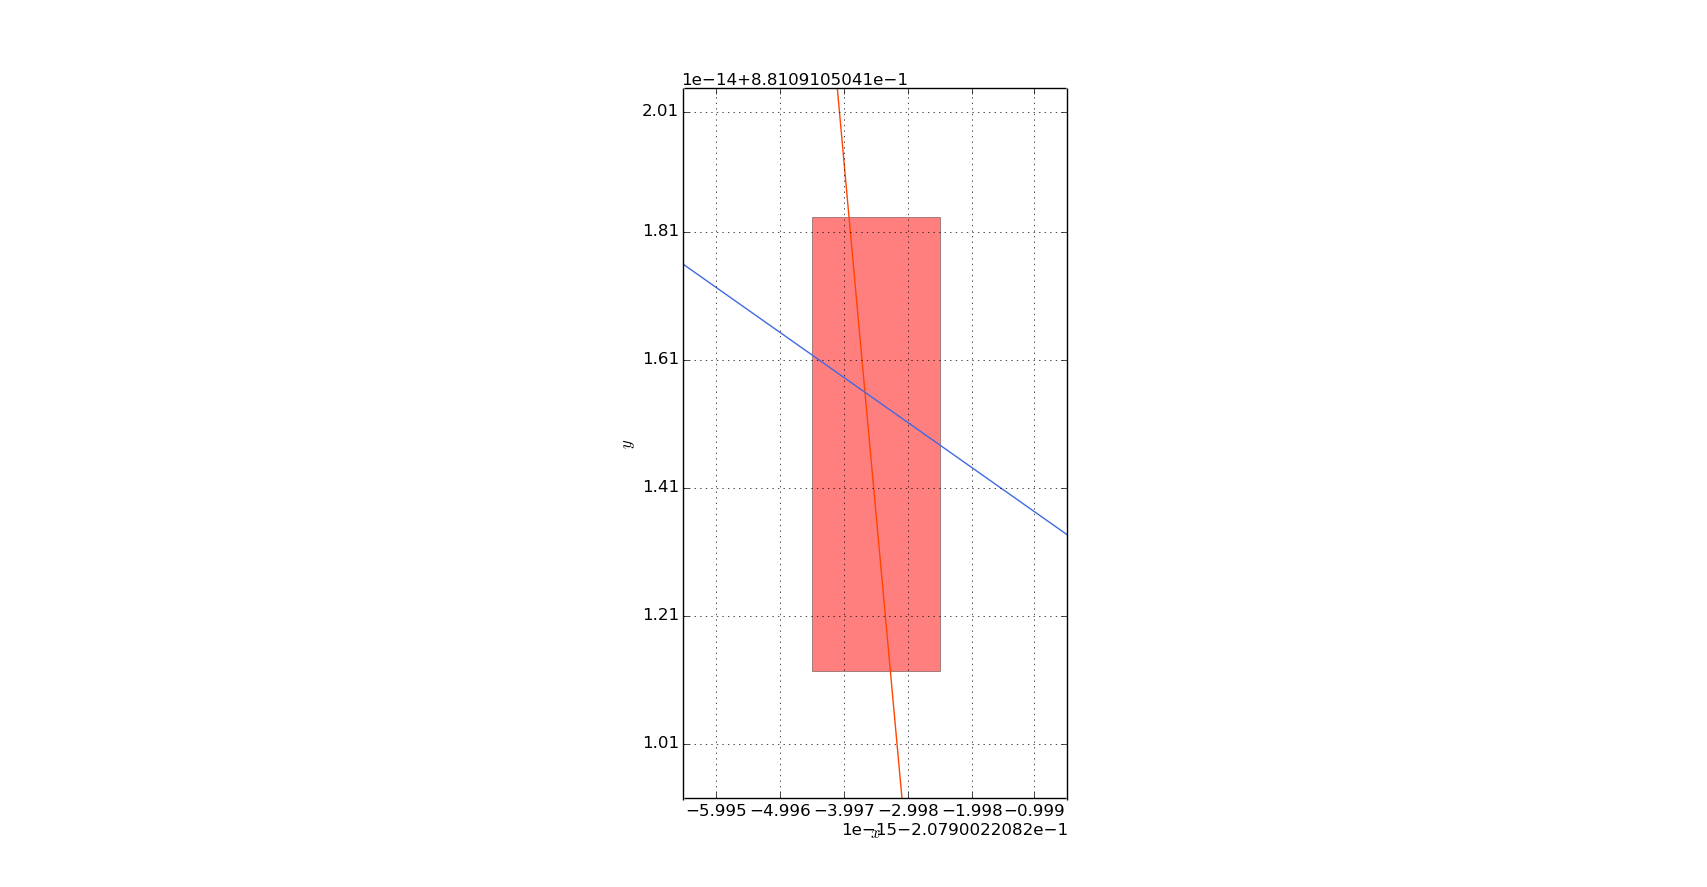
\includegraphics[scale=0.4]{cruce_c}
\caption{Intersección en el intervalo c}
\label{jung_corte3}
\end{figure}



 
%\lhead{\begin{picture}(0,0) \put(0,0){\includegraphics[H][width=20mm]{curvas1}} \end{picture}}

\chapter{Resumen y perspectivas}
Una característica importante a estudiar en los mapeos en general son las variedades estables e inestables asociadas a puntos fijos inestables. En el caso de los mapeos de dos dimensiones resulta manejable, hasta cierto punto, encontrarlas de manera semianalítica usando el método de parametrización. Como se vio el método tiene como núcleo de desarrollo la ecuación de invariancia y la linealización del sistema alrededor de un punto fijo. Sin embargo decir manejable en términos matemáticos y físicos no resulta suficiente si lo que se necesita es estudiar propiedades de los sistemas a partir de las variedades o el comportamiento de puntos fijos. Por ello es que la implementación del método resulta llamativa. Tener un módulo escrito en software libre que calcula las variedades asociadas a puntos fijos hiperbólicos va más allá de generar las relaciones de recurrencia en casos particulares. El método automatizado es capaz de generar las parametrizaciones de las variedades alrededor de un punto fijo hiperbólico conocido, en cualquier mapeo Hamiltoniano de dos dimensiones. La idea detrás de la automatización se basa en que la computadora haga las veces de la recurrencia en lugar de calcularlas de manera analítica. Esto de ninguna manera modifica el modo del método, dando como resultado un método semianalítico con el cual se obtienen las variedades de manera polinomial. \\

Dado que es un método en parte analítico y en parte computacional que involucra series de Taylor; es crucial decir de alguna manera qué tan confiable es la parametrización. Por ello se incluyeron tres formas de evaluar el comportamiento de las variedades, involucrando al error de la solución en serie de la ecuación de invariancia y el estudio de la convergencia mediante dos métodos. Conocer qué tanto es posible afirmar sobre el comportamiento de las variedades depende de estas tres funciones.\\

Los tres ejemplos presentados en el capítulo anterior, presentan comportamientos muy variados: el mapeo estándar tiene una función exponencial además de estar acotado en el espacio fase, mientras en el mapeo exponencial también se tiene una función elemental, pero no está acotado, en el caso de Hénon se tiene un polinomio y no es acotado. El mapeo estándar, por ser bastante conocido, sirvió como referencia para programar el método; el de Hénon por su parte se pensó que sería más fácil de parametrizar, puesto que tiene forma polinomial, lo cual concuerda pues se pudo llegar a valores grandes en el parámetro. En el mapeo exponencial se buscó un reto para el método, pues al ser una función exponencial es más sutil aproximarla por polinomios. Fue notable que en el mapeo de Hénon se pudo observar más sobre las variedades que en los otros dos casos, mientras que el más complicado fue el exponencial. Se puede decir que aquellos mapeos que tengan formas polinomiales serán más dóciles de tratar por el método, debido a que el método consiste en aproximar las variedades por un polinomio.\\

Al explotar el método en los tres mapeos se encontró, con ayuda de los métodos para raíces, los cruces entre variedades para los tres casos, con lo cual se puede saber si hay conexiones homoclínicas o heteroclínicas. Usando aritmética de intervalos se puede tener un método numérico que garantice (matemáticamente hablando), la existencia de puntos homoclínicos o heteroclínicos. En este caso no es estricto el cálculo, pues los coeficientes de la parametrización no son calculados de manera rigurosa con aritmética de intervalos. Esta idea sería una ventana hacia resultados más importantes y amplios, como son el estudio de bifurcaciones y caos topológico.\\

Una característica importante a estudiar también es el comportamiento de los tentáculos formados por las variedades en términos de los parámetros de los mapeos. Como aparece en la sección \ref{SeccionRectanguloFundamental} se pueden obtener tentáculos a partir de iterar la parametrización mediante el mapeo. Así se puede calcular un polinomio de orden no tan grande, dependiendo del mapeo, e iterando hasta llegar a estructuras difíciles de alcanzar sólo con la parametrización.\\

Una de las dudas que surgió durante el proceso de este trabajo se formuló en principio como sigue: ¿es posible reparametrizar a partir de un cierto punto la variedad?. Por ejemplo en los casos en los que se tienen puntos homoclínicos, se quisiera comenzar una nueva parametrización a partir del mismo. Esto permitiría construir las variedades por pedazos en los que se tenga un error más controlable y por tanto tener una mayor parte de la misma. Otra de las preguntas que surgieron tiene que ver con los polinomios de Chebyshev. Los polinomios de Taylor no tienen una dirección preferencial en el plano complejo, mientras que los de Chebyshev sí la tienen; el tener una dirección preferencial puede servir para mejorar el error y conseguir un polinomio que describa mejor la variedad a valores grandes del parámetro. 
     % ~20 páginas - Explicar el problema en específico que se va a resolver, la met   % ~20 páginas - Presentar los resultados tal cual son, y analizarlos.
%\relax 
\providecommand\hyper@newdestlabel[2]{}
\FN@pp@footnotehinttrue 
\@setckpt{Capitulo5/Bifurcaci\unhbox \voidb@x \bgroup \let \unhbox \voidb@x \setbox \@tempboxa \hbox {o\global \mathchardef \accent@spacefactor \spacefactor }\accent 19 o\egroup \spacefactor \accent@spacefactor \futurelet \@let@token \penalty \@M \hskip \z@skip n}{
\setcounter{page}{7}
\setcounter{equation}{0}
\setcounter{enumi}{0}
\setcounter{enumii}{0}
\setcounter{enumiii}{0}
\setcounter{enumiv}{0}
\setcounter{footnote}{0}
\setcounter{mpfootnote}{0}
\setcounter{part}{0}
\setcounter{chapter}{0}
\setcounter{section}{0}
\setcounter{subsection}{0}
\setcounter{subsubsection}{0}
\setcounter{paragraph}{0}
\setcounter{subparagraph}{0}
\setcounter{figure}{0}
\setcounter{table}{0}
\setcounter{parentequation}{0}
\setcounter{lstnumber}{1}
\setcounter{ContinuedFloat}{0}
\setcounter{subfigure}{0}
\setcounter{lofdepth}{1}
\setcounter{subtable}{0}
\setcounter{lotdepth}{1}
\setcounter{float@type}{8}
\setcounter{pp@next@reset}{1}
\setcounter{@fnserial}{0}
\setcounter{NAT@ctr}{0}
\setcounter{Item}{0}
\setcounter{Hfootnote}{0}
\setcounter{bookmark@seq@number}{2}
\setcounter{blindtext}{1}
\setcounter{Blindtext}{5}
\setcounter{blind@countparstart}{0}
\setcounter{blindlist}{0}
\setcounter{blindlistlevel}{0}
\setcounter{blindlist@level}{0}
\setcounter{blind@listcount}{0}
\setcounter{blind@levelcount}{0}
\setcounter{blind@randomcount}{0}
\setcounter{blind@randommax}{1}
\setcounter{blind@pangramcount}{0}
\setcounter{blind@pangrammax}{1}
\setcounter{lstlisting}{0}
\setcounter{section@level}{0}
}
            % ~5 páginas - Resumir lo que se hizo y lo que no y comentar trabajos futuros sobre el tema

%%%%%%%%%%%%%%%%%%%%%%%%%%%%%%%%%%%%%%%%%%%%%%%%%%%%%
%                   APÉNDICES                       %
%%%%%%%%%%%%%%%%%%%%%%%%%%%%%%%%%%%%%%%%%%%%%%%%%%%%%
\appendix
%% this file is called up by thesis.tex
% content in this file will be fed into the main document
\chapter{Código }
% top level followed by section, subsection

\section{Método de Parametrización}
A continuación presentamos el código escrito en Julia , sólo con el fin de apoyar en alguna parte de la lectura del pseudocóigo ya que el mismo se encuentra en el repositorio de GitHub PONER-LIGA y se puede consultar en internet.

               % Colocar los circuitos, manuales, código fuente, pruebas de teoremas, etc.

%%%%%%%%%%%%%%%%%%%%%%%%%%%%%%%%%%%%%%%%%%%%%%%%%%%%%
%                   REFERENCIAS                     %
%%%%%%%%%%%%%%%%%%%%%%%%%%%%%%%%%%%%%%%%%%%%%%%%%%%%%
% existen varios estilos de bilbiografía, pueden cambiarlos a placer
 % otros estilos pueden ser abbrv, acm, alpha, apalike, ieeetr, plain, siam, unsrt

%El formato trae otros estilos, o pueden agregar uno que les guste:
%\bibliographystyle{Latex/Classes/PhDbiblio-case} % title forced lower case
%\bibliographystyle{Latex/Classes/PhDbiblio-bold} % title as in bibtex but bold
%\bibliographystyle{Latex/Classes/PhDbiblio-url} % bold + www link if provided
%\bibliographystyle{Latex/Classes/jmb} % calls style file jmb.bst
\bibliographystyle{unsrt}
\bibliography{referencias}             % Archivo .bib
\nocite{*}
\end{document}
